\documentclass[11pt]{article}
% Journal-neutral preprint layout. For submission, move the sections into the target
% journal's template (e.g. elsarticle for Energy and Buildings / J. Building Engineering).
\usepackage[a4paper,margin=2.3cm]{geometry}
\usepackage{amsmath,amssymb,graphicx,booktabs,xcolor}
\usepackage[hidelinks]{hyperref}
\graphicspath{{../../results/figures/}}
% generated by make_numbers.py -- do not edit
\newcommand{\ETh}{5{,}028}
\newcommand{\EThCI}{1}
\newcommand{\CostTh}{36{,}950}
\newcommand{\CostThCI}{8}
\newcommand{\KhTh}{1{,}102}
\newcommand{\KhThCI}{3}
\newcommand{\KhOverTh}{91}
\newcommand{\KhOverThCI}{1}
\newcommand{\KhColdTh}{1{,}011}
\newcommand{\KhColdThCI}{3}
\newcommand{\AccTh}{82.7}
\newcommand{\AccThCI}{0.1}
\newcommand{\RmseTh}{1.17}
\newcommand{\RmseThCI}{0.00}
\newcommand{\PeakTh}{3.38}
\newcommand{\PeakThCI}{0.01}
\newcommand{\StartsTh}{8{,}476}
\newcommand{\StartsThCI}{26}
\newcommand{\EvrfTh}{3{,}224}
\newcommand{\EvrfThCI}{1}
\newcommand{\CarbonTh}{3{,}655}
\newcommand{\CarbonThCI}{1}
\newcommand{\PeakShareTh}{34.2}
\newcommand{\MsTh}{--}
\newcommand{\dCostTh}{+0.0}
\newcommand{\dCostThabs}{0.0}
\newcommand{\dETh}{+0.0}
\newcommand{\dEThabs}{0.0}
\newcommand{\dKhTh}{+0.0}
\newcommand{\dKhThabs}{0.0}
\newcommand{\CostSaveTh}{0}
\newcommand{\EPid}{5{,}403}
\newcommand{\EPidCI}{0}
\newcommand{\CostPid}{39{,}460}
\newcommand{\CostPidCI}{3}
\newcommand{\KhPid}{315}
\newcommand{\KhPidCI}{0}
\newcommand{\KhOverPid}{14}
\newcommand{\KhOverPidCI}{0}
\newcommand{\KhColdPid}{302}
\newcommand{\KhColdPidCI}{0}
\newcommand{\AccPid}{94.8}
\newcommand{\AccPidCI}{0.0}
\newcommand{\RmsePid}{0.75}
\newcommand{\RmsePidCI}{0.00}
\newcommand{\PeakPid}{2.69}
\newcommand{\PeakPidCI}{0.04}
\newcommand{\StartsPid}{488}
\newcommand{\StartsPidCI}{13}
\newcommand{\EvrfPid}{3{,}449}
\newcommand{\EvrfPidCI}{1}
\newcommand{\CarbonPid}{3{,}928}
\newcommand{\CarbonPidCI}{0}
\newcommand{\PeakSharePid}{34.4}
\newcommand{\MsPid}{--}
\newcommand{\dCostPid}{+6.8}
\newcommand{\dCostPidabs}{6.8}
\newcommand{\dEPid}{+7.5}
\newcommand{\dEPidabs}{7.5}
\newcommand{\dKhPid}{-71.4}
\newcommand{\dKhPidabs}{71.4}
\newcommand{\CostSavePid}{-2{,}510}
\newcommand{\EMpc}{5{,}243}
\newcommand{\EMpcCI}{3}
\newcommand{\CostMpc}{38{,}306}
\newcommand{\CostMpcCI}{26}
\newcommand{\KhMpc}{251}
\newcommand{\KhMpcCI}{2}
\newcommand{\KhOverMpc}{97}
\newcommand{\KhOverMpcCI}{2}
\newcommand{\KhColdMpc}{154}
\newcommand{\KhColdMpcCI}{1}
\newcommand{\AccMpc}{95.7}
\newcommand{\AccMpcCI}{0.0}
\newcommand{\RmseMpc}{0.99}
\newcommand{\RmseMpcCI}{0.00}
\newcommand{\PeakMpc}{2.78}
\newcommand{\PeakMpcCI}{0.07}
\newcommand{\StartsMpc}{337}
\newcommand{\StartsMpcCI}{5}
\newcommand{\EvrfMpc}{3{,}244}
\newcommand{\EvrfMpcCI}{3}
\newcommand{\CarbonMpc}{3{,}811}
\newcommand{\CarbonMpcCI}{2}
\newcommand{\PeakShareMpc}{34.2}
\newcommand{\MsMpc}{26}
\newcommand{\dCostMpc}{+3.7}
\newcommand{\dCostMpcabs}{3.7}
\newcommand{\dEMpc}{+4.3}
\newcommand{\dEMpcabs}{4.3}
\newcommand{\dKhMpc}{-77.3}
\newcommand{\dKhMpcabs}{77.3}
\newcommand{\CostSaveMpc}{-1{,}357}
\newcommand{\EDqn}{5{,}273}
\newcommand{\EDqnCI}{112}
\newcommand{\CostDqn}{38{,}799}
\newcommand{\CostDqnCI}{682}
\newcommand{\KhDqn}{259}
\newcommand{\KhDqnCI}{54}
\newcommand{\KhOverDqn}{30}
\newcommand{\KhOverDqnCI}{17}
\newcommand{\KhColdDqn}{229}
\newcommand{\KhColdDqnCI}{64}
\newcommand{\AccDqn}{94.3}
\newcommand{\AccDqnCI}{0.8}
\newcommand{\RmseDqn}{0.90}
\newcommand{\RmseDqnCI}{0.04}
\newcommand{\PeakDqn}{3.32}
\newcommand{\PeakDqnCI}{0.07}
\newcommand{\StartsDqn}{4{,}897}
\newcommand{\StartsDqnCI}{978}
\newcommand{\EvrfDqn}{3{,}422}
\newcommand{\EvrfDqnCI}{83}
\newcommand{\CarbonDqn}{3{,}833}
\newcommand{\CarbonDqnCI}{81}
\newcommand{\PeakShareDqn}{34.7}
\newcommand{\MsDqn}{--}
\newcommand{\dCostDqn}{+5.0}
\newcommand{\dCostDqnabs}{5.0}
\newcommand{\dEDqn}{+4.9}
\newcommand{\dEDqnabs}{4.9}
\newcommand{\dKhDqn}{-76.5}
\newcommand{\dKhDqnabs}{76.5}
\newcommand{\CostSaveDqn}{-1{,}850}
\newcommand{\EHyb}{5{,}198}
\newcommand{\EHybCI}{1}
\newcommand{\CostHyb}{38{,}005}
\newcommand{\CostHybCI}{14}
\newcommand{\KhHyb}{185}
\newcommand{\KhHybCI}{1}
\newcommand{\KhOverHyb}{37}
\newcommand{\KhOverHybCI}{1}
\newcommand{\KhColdHyb}{148}
\newcommand{\KhColdHybCI}{1}
\newcommand{\AccHyb}{96.1}
\newcommand{\AccHybCI}{0.0}
\newcommand{\RmseHyb}{0.99}
\newcommand{\RmseHybCI}{0.00}
\newcommand{\PeakHyb}{2.78}
\newcommand{\PeakHybCI}{0.10}
\newcommand{\StartsHyb}{750}
\newcommand{\StartsHybCI}{19}
\newcommand{\EvrfHyb}{3{,}195}
\newcommand{\EvrfHybCI}{1}
\newcommand{\CarbonHyb}{3{,}779}
\newcommand{\CarbonHybCI}{1}
\newcommand{\PeakShareHyb}{34.5}
\newcommand{\MsHyb}{26}
\newcommand{\dCostHyb}{+2.9}
\newcommand{\dCostHybabs}{2.9}
\newcommand{\dEHyb}{+3.4}
\newcommand{\dEHybabs}{3.4}
\newcommand{\dKhHyb}{-83.2}
\newcommand{\dKhHybabs}{83.2}
\newcommand{\CostSaveHyb}{-1{,}055}
\newcommand{\RelHybPidCost}{3.7}
\newcommand{\RelHybPidCostSigned}{-3.7}
\newcommand{\RelHybPidKh}{41.3}
\newcommand{\RelHybPidKhSigned}{-41.3}
\newcommand{\RelHybPidE}{3.8}
\newcommand{\RelHybPidESigned}{-3.8}
\newcommand{\RelHybMpcCost}{0.8}
\newcommand{\RelHybMpcCostSigned}{-0.8}
\newcommand{\RelHybMpcKh}{26.1}
\newcommand{\RelHybMpcKhSigned}{-26.1}
\newcommand{\RelHybMpcE}{0.9}
\newcommand{\RelHybMpcESigned}{-0.9}
\newcommand{\RelMpcPidCost}{2.9}
\newcommand{\RelMpcPidCostSigned}{-2.9}
\newcommand{\RelMpcPidKh}{20.5}
\newcommand{\RelMpcPidKhSigned}{-20.5}
\newcommand{\RelMpcPidE}{3.0}
\newcommand{\RelMpcPidESigned}{-3.0}
\newcommand{\RelDqnPidCost}{1.7}
\newcommand{\RelDqnPidCostSigned}{-1.7}
\newcommand{\RelDqnPidKh}{17.8}
\newcommand{\RelDqnPidKhSigned}{-17.8}
\newcommand{\RelDqnPidE}{2.4}
\newcommand{\RelDqnPidESigned}{-2.4}
\newcommand{\RelHybDqnCost}{2.0}
\newcommand{\RelHybDqnCostSigned}{-2.0}
\newcommand{\RelHybDqnKh}{28.6}
\newcommand{\RelHybDqnKhSigned}{-28.6}
\newcommand{\RelHybDqnE}{1.4}
\newcommand{\RelHybDqnESigned}{-1.4}
\newcommand{\StartsRatioTh}{11}
\newcommand{\PairHybridMpcCost}{-304}
\newcommand{\PairHybridMpcCostLo}{-387}
\newcommand{\PairHybridMpcCostHi}{-232}
\newcommand{\PairHybridMpcCostP}{<0.001}
\newcommand{\PairHybridMpcKh}{-67}
\newcommand{\PairHybridMpcKhLo}{-99}
\newcommand{\PairHybridMpcKhHi}{-40}
\newcommand{\PairHybridMpcKhP}{<0.001}
\newcommand{\PairHybridMpcE}{-45}
\newcommand{\PairHybridMpcELo}{-57}
\newcommand{\PairHybridMpcEHi}{-35}
\newcommand{\PairHybridMpcEP}{<0.001}
\newcommand{\PairHybridPidCost}{-1{,}447}
\newcommand{\PairHybridPidCostLo}{-1{,}579}
\newcommand{\PairHybridPidCostHi}{-1{,}308}
\newcommand{\PairHybridPidCostP}{<0.001}
\newcommand{\PairHybridPidKh}{-130}
\newcommand{\PairHybridPidKhLo}{-219}
\newcommand{\PairHybridPidKhHi}{-46}
\newcommand{\PairHybridPidKhP}{<0.001}
\newcommand{\PairHybridPidE}{-205}
\newcommand{\PairHybridPidELo}{-232}
\newcommand{\PairHybridPidEHi}{-175}
\newcommand{\PairHybridPidEP}{<0.001}
\newcommand{\PairMpcPidCost}{-1{,}144}
\newcommand{\PairMpcPidCostLo}{-1{,}287}
\newcommand{\PairMpcPidCostHi}{-991}
\newcommand{\PairMpcPidCostP}{<0.001}
\newcommand{\PairMpcPidKh}{-63}
\newcommand{\PairMpcPidKhLo}{-158}
\newcommand{\PairMpcPidKhHi}{28}
\newcommand{\PairMpcPidKhP}{0.248}
\newcommand{\PairMpcPidE}{-160}
\newcommand{\PairMpcPidELo}{-187}
\newcommand{\PairMpcPidEHi}{-130}
\newcommand{\PairMpcPidEP}{<0.001}
\newcommand{\PairRlPidCost}{-1{,}281}
\newcommand{\PairRlPidCostLo}{-1{,}884}
\newcommand{\PairRlPidCostHi}{-582}
\newcommand{\PairRlPidCostP}{<0.001}
\newcommand{\PairRlPidKh}{-110}
\newcommand{\PairRlPidKhLo}{-203}
\newcommand{\PairRlPidKhHi}{-32}
\newcommand{\PairRlPidKhP}{0.844}
\newcommand{\PairRlPidE}{-219}
\newcommand{\PairRlPidELo}{-302}
\newcommand{\PairRlPidEHi}{-125}
\newcommand{\PairRlPidEP}{<0.001}
\newcommand{\PairPidThermostatCost}{2{,}508}
\newcommand{\PairPidThermostatCostLo}{2{,}024}
\newcommand{\PairPidThermostatCostHi}{3{,}028}
\newcommand{\PairPidThermostatCostP}{<0.001}
\newcommand{\PairPidThermostatKh}{-788}
\newcommand{\PairPidThermostatKhLo}{-825}
\newcommand{\PairPidThermostatKhHi}{-757}
\newcommand{\PairPidThermostatKhP}{<0.001}
\newcommand{\PairPidThermostatE}{374}
\newcommand{\PairPidThermostatELo}{305}
\newcommand{\PairPidThermostatEHi}{448}
\newcommand{\PairPidThermostatEP}{<0.001}
\newcommand{\PairMpcThermostatCost}{1{,}364}
\newcommand{\PairMpcThermostatCostLo}{879}
\newcommand{\PairMpcThermostatCostHi}{1{,}893}
\newcommand{\PairMpcThermostatCostP}{<0.001}
\newcommand{\PairMpcThermostatKh}{-851}
\newcommand{\PairMpcThermostatKhLo}{-958}
\newcommand{\PairMpcThermostatKhHi}{-748}
\newcommand{\PairMpcThermostatKhP}{<0.001}
\newcommand{\PairMpcThermostatE}{214}
\newcommand{\PairMpcThermostatELo}{152}
\newcommand{\PairMpcThermostatEHi}{285}
\newcommand{\PairMpcThermostatEP}{<0.001}
\newcommand{\PairRlThermostatCost}{1{,}227}
\newcommand{\PairRlThermostatCostLo}{709}
\newcommand{\PairRlThermostatCostHi}{1{,}815}
\newcommand{\PairRlThermostatCostP}{<0.001}
\newcommand{\PairRlThermostatKh}{-898}
\newcommand{\PairRlThermostatKhLo}{-1{,}000}
\newcommand{\PairRlThermostatKhHi}{-815}
\newcommand{\PairRlThermostatKhP}{<0.001}
\newcommand{\PairRlThermostatE}{155}
\newcommand{\PairRlThermostatELo}{87}
\newcommand{\PairRlThermostatEHi}{231}
\newcommand{\PairRlThermostatEP}{<0.001}
\newcommand{\PairHybridThermostatCost}{1{,}061}
\newcommand{\PairHybridThermostatCostLo}{530}
\newcommand{\PairHybridThermostatCostHi}{1{,}673}
\newcommand{\PairHybridThermostatCostP}{<0.001}
\newcommand{\PairHybridThermostatKh}{-918}
\newcommand{\PairHybridThermostatKhLo}{-1{,}021}
\newcommand{\PairHybridThermostatKhHi}{-836}
\newcommand{\PairHybridThermostatKhP}{<0.001}
\newcommand{\PairHybridThermostatE}{169}
\newcommand{\PairHybridThermostatELo}{97}
\newcommand{\PairHybridThermostatEHi}{249}
\newcommand{\PairHybridThermostatEP}{<0.001}
\newcommand{\SBaseETh}{5{,}029}
\newcommand{\SBaseCostTh}{36{,}953}
\newcommand{\SBaseKhTh}{1{,}103}
\newcommand{\SBaseAccTh}{82.6}
\newcommand{\SBaseCoTh}{643}
\newcommand{\SBaseCoHTh}{0}
\newcommand{\SBasePmTh}{13.0}
\newcommand{\SBasePmDTh}{102}
\newcommand{\SBasePmDsixtyTh}{0}
\newcommand{\SBaseRhTh}{371}
\newcommand{\SBasePkShTh}{0.341}
\newcommand{\SBaseEPid}{5{,}403}
\newcommand{\SBaseCostPid}{39{,}461}
\newcommand{\SBaseKhPid}{315}
\newcommand{\SBaseAccPid}{94.8}
\newcommand{\SBaseCoPid}{640}
\newcommand{\SBaseCoHPid}{0}
\newcommand{\SBasePmPid}{13.5}
\newcommand{\SBasePmDPid}{136}
\newcommand{\SBasePmDsixtyPid}{0}
\newcommand{\SBaseRhPid}{316}
\newcommand{\SBasePkShPid}{0.344}
\newcommand{\SBaseEMpc}{5{,}243}
\newcommand{\SBaseCostMpc}{38{,}317}
\newcommand{\SBaseKhMpc}{252}
\newcommand{\SBaseAccMpc}{95.6}
\newcommand{\SBaseCoMpc}{640}
\newcommand{\SBaseCoHMpc}{0}
\newcommand{\SBasePmMpc}{13.5}
\newcommand{\SBasePmDMpc}{132}
\newcommand{\SBasePmDsixtyMpc}{0}
\newcommand{\SBaseRhMpc}{225}
\newcommand{\SBasePkShMpc}{0.342}
\newcommand{\SBaseEDqn}{5{,}184}
\newcommand{\SBaseCostDqn}{38{,}180}
\newcommand{\SBaseKhDqn}{205}
\newcommand{\SBaseAccDqn}{94.7}
\newcommand{\SBaseCoDqn}{642}
\newcommand{\SBaseCoHDqn}{0}
\newcommand{\SBasePmDqn}{13.2}
\newcommand{\SBasePmDDqn}{110}
\newcommand{\SBasePmDsixtyDqn}{0}
\newcommand{\SBaseRhDqn}{400}
\newcommand{\SBasePkShDqn}{0.350}
\newcommand{\SBaseEHyb}{5{,}198}
\newcommand{\SBaseCostHyb}{38{,}014}
\newcommand{\SBaseKhHyb}{185}
\newcommand{\SBaseAccHyb}{96.1}
\newcommand{\SBaseCoHyb}{640}
\newcommand{\SBaseCoHHyb}{0}
\newcommand{\SBasePmHyb}{13.5}
\newcommand{\SBasePmDHyb}{135}
\newcommand{\SBasePmDsixtyHyb}{0}
\newcommand{\SBaseRhHyb}{220}
\newcommand{\SBasePkShHyb}{0.345}
\newcommand{\SHeatETh}{6{,}723}
\newcommand{\SHeatCostTh}{49{,}405}
\newcommand{\SHeatKhTh}{673}
\newcommand{\SHeatAccTh}{87.2}
\newcommand{\SHeatCoTh}{634}
\newcommand{\SHeatCoHTh}{0}
\newcommand{\SHeatPmTh}{13.7}
\newcommand{\SHeatPmDTh}{157}
\newcommand{\SHeatPmDsixtyTh}{0}
\newcommand{\SHeatRhTh}{0}
\newcommand{\SHeatPkShTh}{0.331}
\newcommand{\SHeatEPid}{7{,}061}
\newcommand{\SHeatCostPid}{51{,}616}
\newcommand{\SHeatKhPid}{65}
\newcommand{\SHeatAccPid}{98.4}
\newcommand{\SHeatCoPid}{629}
\newcommand{\SHeatCoHPid}{0}
\newcommand{\SHeatPmPid}{14.6}
\newcommand{\SHeatPmDPid}{166}
\newcommand{\SHeatPmDsixtyPid}{0}
\newcommand{\SHeatRhPid}{0}
\newcommand{\SHeatPkShPid}{0.335}
\newcommand{\SHeatEMpc}{7{,}020}
\newcommand{\SHeatCostMpc}{51{,}135}
\newcommand{\SHeatKhMpc}{126}
\newcommand{\SHeatAccMpc}{98.0}
\newcommand{\SHeatCoMpc}{629}
\newcommand{\SHeatCoHMpc}{0}
\newcommand{\SHeatPmMpc}{14.5}
\newcommand{\SHeatPmDMpc}{167}
\newcommand{\SHeatPmDsixtyMpc}{0}
\newcommand{\SHeatRhMpc}{0}
\newcommand{\SHeatPkShMpc}{0.327}
\newcommand{\SHeatEDqn}{7{,}032}
\newcommand{\SHeatCostDqn}{51{,}791}
\newcommand{\SHeatKhDqn}{109}
\newcommand{\SHeatAccDqn}{96.2}
\newcommand{\SHeatCoDqn}{632}
\newcommand{\SHeatCoHDqn}{0}
\newcommand{\SHeatPmDqn}{14.0}
\newcommand{\SHeatPmDDqn}{152}
\newcommand{\SHeatPmDsixtyDqn}{0}
\newcommand{\SHeatRhDqn}{0}
\newcommand{\SHeatPkShDqn}{0.341}
\newcommand{\SHeatEHyb}{6{,}971}
\newcommand{\SHeatCostHyb}{50{,}788}
\newcommand{\SHeatKhHyb}{52}
\newcommand{\SHeatAccHyb}{98.7}
\newcommand{\SHeatCoHyb}{629}
\newcommand{\SHeatCoHHyb}{0}
\newcommand{\SHeatPmHyb}{14.6}
\newcommand{\SHeatPmDHyb}{167}
\newcommand{\SHeatPmDsixtyHyb}{0}
\newcommand{\SHeatRhHyb}{0}
\newcommand{\SHeatPkShHyb}{0.328}
\newcommand{\SMassLoETh}{5{,}207}
\newcommand{\SMassLoCostTh}{38{,}602}
\newcommand{\SMassLoKhTh}{1{,}990}
\newcommand{\SMassLoAccTh}{79.1}
\newcommand{\SMassLoCoTh}{643}
\newcommand{\SMassLoCoHTh}{0}
\newcommand{\SMassLoPmTh}{13.1}
\newcommand{\SMassLoPmDTh}{112}
\newcommand{\SMassLoPmDsixtyTh}{0}
\newcommand{\SMassLoRhTh}{1{,}182}
\newcommand{\SMassLoPkShTh}{0.315}
\newcommand{\SMassLoEPid}{5{,}498}
\newcommand{\SMassLoCostPid}{40{,}583}
\newcommand{\SMassLoKhPid}{1{,}380}
\newcommand{\SMassLoAccPid}{87.8}
\newcommand{\SMassLoCoPid}{640}
\newcommand{\SMassLoCoHPid}{0}
\newcommand{\SMassLoPmPid}{13.6}
\newcommand{\SMassLoPmDPid}{141}
\newcommand{\SMassLoPmDsixtyPid}{0}
\newcommand{\SMassLoRhPid}{1{,}138}
\newcommand{\SMassLoPkShPid}{0.336}
\newcommand{\SMassLoEMpc}{5{,}387}
\newcommand{\SMassLoCostMpc}{39{,}705}
\newcommand{\SMassLoKhMpc}{1{,}100}
\newcommand{\SMassLoAccMpc}{87.6}
\newcommand{\SMassLoCoMpc}{640}
\newcommand{\SMassLoCoHMpc}{0}
\newcommand{\SMassLoPmMpc}{13.5}
\newcommand{\SMassLoPmDMpc}{133}
\newcommand{\SMassLoPmDsixtyMpc}{0}
\newcommand{\SMassLoRhMpc}{1{,}041}
\newcommand{\SMassLoPkShMpc}{0.309}
\newcommand{\SMassLoEDqn}{5{,}326}
\newcommand{\SMassLoCostDqn}{39{,}514}
\newcommand{\SMassLoKhDqn}{1{,}145}
\newcommand{\SMassLoAccDqn}{85.1}
\newcommand{\SMassLoCoDqn}{641}
\newcommand{\SMassLoCoHDqn}{0}
\newcommand{\SMassLoPmDqn}{13.3}
\newcommand{\SMassLoPmDDqn}{119}
\newcommand{\SMassLoPmDsixtyDqn}{0}
\newcommand{\SMassLoRhDqn}{1{,}227}
\newcommand{\SMassLoPkShDqn}{0.326}
\newcommand{\SMassLoEHyb}{5{,}347}
\newcommand{\SMassLoCostHyb}{39{,}423}
\newcommand{\SMassLoKhHyb}{972}
\newcommand{\SMassLoAccHyb}{88.2}
\newcommand{\SMassLoCoHyb}{640}
\newcommand{\SMassLoCoHHyb}{0}
\newcommand{\SMassLoPmHyb}{13.5}
\newcommand{\SMassLoPmDHyb}{136}
\newcommand{\SMassLoPmDsixtyHyb}{0}
\newcommand{\SMassLoRhHyb}{1{,}027}
\newcommand{\SMassLoPkShHyb}{0.310}
\newcommand{\SMassHiETh}{4{,}946}
\newcommand{\SMassHiCostTh}{36{,}089}
\newcommand{\SMassHiKhTh}{864}
\newcommand{\SMassHiAccTh}{84.8}
\newcommand{\SMassHiCoTh}{643}
\newcommand{\SMassHiCoHTh}{0}
\newcommand{\SMassHiPmTh}{12.9}
\newcommand{\SMassHiPmDTh}{95}
\newcommand{\SMassHiPmDsixtyTh}{0}
\newcommand{\SMassHiRhTh}{77}
\newcommand{\SMassHiPkShTh}{0.338}
\newcommand{\SMassHiEPid}{5{,}363}
\newcommand{\SMassHiCostPid}{38{,}961}
\newcommand{\SMassHiKhPid}{83}
\newcommand{\SMassHiAccPid}{97.8}
\newcommand{\SMassHiCoPid}{640}
\newcommand{\SMassHiCoHPid}{0}
\newcommand{\SMassHiPmPid}{13.5}
\newcommand{\SMassHiPmDPid}{135}
\newcommand{\SMassHiPmDsixtyPid}{0}
\newcommand{\SMassHiRhPid}{43}
\newcommand{\SMassHiPkShPid}{0.336}
\newcommand{\SMassHiEMpc}{5{,}141}
\newcommand{\SMassHiCostMpc}{37{,}529}
\newcommand{\SMassHiKhMpc}{99}
\newcommand{\SMassHiAccMpc}{98.0}
\newcommand{\SMassHiCoMpc}{640}
\newcommand{\SMassHiCoHMpc}{0}
\newcommand{\SMassHiPmMpc}{13.5}
\newcommand{\SMassHiPmDMpc}{136}
\newcommand{\SMassHiPmDsixtyMpc}{0}
\newcommand{\SMassHiRhMpc}{19}
\newcommand{\SMassHiPkShMpc}{0.356}
\newcommand{\SMassHiEDqn}{5{,}124}
\newcommand{\SMassHiCostDqn}{37{,}511}
\newcommand{\SMassHiKhDqn}{58}
\newcommand{\SMassHiAccDqn}{97.9}
\newcommand{\SMassHiCoDqn}{642}
\newcommand{\SMassHiCoHDqn}{0}
\newcommand{\SMassHiPmDqn}{13.1}
\newcommand{\SMassHiPmDDqn}{108}
\newcommand{\SMassHiPmDsixtyDqn}{0}
\newcommand{\SMassHiRhDqn}{74}
\newcommand{\SMassHiPkShDqn}{0.348}
\newcommand{\SMassHiEHyb}{5{,}112}
\newcommand{\SMassHiCostHyb}{37{,}338}
\newcommand{\SMassHiKhHyb}{53}
\newcommand{\SMassHiAccHyb}{98.5}
\newcommand{\SMassHiCoHyb}{639}
\newcommand{\SMassHiCoHHyb}{0}
\newcommand{\SMassHiPmHyb}{13.5}
\newcommand{\SMassHiPmDHyb}{132}
\newcommand{\SMassHiPmDsixtyHyb}{0}
\newcommand{\SMassHiRhHyb}{19}
\newcommand{\SMassHiPkShHyb}{0.359}
\newcommand{\SFlatETh}{5{,}029}
\newcommand{\SFlatCostTh}{35{,}957}
\newcommand{\SFlatKhTh}{1{,}103}
\newcommand{\SFlatAccTh}{82.6}
\newcommand{\SFlatCoTh}{643}
\newcommand{\SFlatCoHTh}{0}
\newcommand{\SFlatPmTh}{13.0}
\newcommand{\SFlatPmDTh}{102}
\newcommand{\SFlatPmDsixtyTh}{0}
\newcommand{\SFlatRhTh}{371}
\newcommand{\SFlatPkShTh}{1.000}
\newcommand{\SFlatEPid}{5{,}403}
\newcommand{\SFlatCostPid}{38{,}630}
\newcommand{\SFlatKhPid}{315}
\newcommand{\SFlatAccPid}{94.8}
\newcommand{\SFlatCoPid}{640}
\newcommand{\SFlatCoHPid}{0}
\newcommand{\SFlatPmPid}{13.5}
\newcommand{\SFlatPmDPid}{136}
\newcommand{\SFlatPmDsixtyPid}{0}
\newcommand{\SFlatRhPid}{316}
\newcommand{\SFlatPkShPid}{1.000}
\newcommand{\SFlatEMpc}{5{,}226}
\newcommand{\SFlatCostMpc}{37{,}367}
\newcommand{\SFlatKhMpc}{251}
\newcommand{\SFlatAccMpc}{95.7}
\newcommand{\SFlatCoMpc}{640}
\newcommand{\SFlatCoHMpc}{0}
\newcommand{\SFlatPmMpc}{13.5}
\newcommand{\SFlatPmDMpc}{132}
\newcommand{\SFlatPmDsixtyMpc}{0}
\newcommand{\SFlatRhMpc}{226}
\newcommand{\SFlatPkShMpc}{1.000}
\newcommand{\SFlatEDqn}{5{,}161}
\newcommand{\SFlatCostDqn}{36{,}903}
\newcommand{\SFlatKhDqn}{193}
\newcommand{\SFlatAccDqn}{94.7}
\newcommand{\SFlatCoDqn}{642}
\newcommand{\SFlatCoHDqn}{0}
\newcommand{\SFlatPmDqn}{13.2}
\newcommand{\SFlatPmDDqn}{109}
\newcommand{\SFlatPmDsixtyDqn}{0}
\newcommand{\SFlatRhDqn}{372}
\newcommand{\SFlatPkShDqn}{1.000}
\newcommand{\SFlatEHyb}{5{,}180}
\newcommand{\SFlatCostHyb}{37{,}037}
\newcommand{\SFlatKhHyb}{185}
\newcommand{\SFlatAccHyb}{96.1}
\newcommand{\SFlatCoHyb}{640}
\newcommand{\SFlatCoHHyb}{0}
\newcommand{\SFlatPmHyb}{13.5}
\newcommand{\SFlatPmDHyb}{134}
\newcommand{\SFlatPmDsixtyHyb}{0}
\newcommand{\SFlatRhHyb}{219}
\newcommand{\SFlatPkShHyb}{1.000}
\newcommand{\SNoMisETh}{4{,}736}
\newcommand{\SNoMisCostTh}{34{,}669}
\newcommand{\SNoMisKhTh}{1{,}397}
\newcommand{\SNoMisAccTh}{80.2}
\newcommand{\SNoMisCoTh}{644}
\newcommand{\SNoMisCoHTh}{0}
\newcommand{\SNoMisPmTh}{12.9}
\newcommand{\SNoMisPmDTh}{92}
\newcommand{\SNoMisPmDsixtyTh}{0}
\newcommand{\SNoMisRhTh}{379}
\newcommand{\SNoMisPkShTh}{0.338}
\newcommand{\SNoMisEPid}{5{,}132}
\newcommand{\SNoMisCostPid}{37{,}346}
\newcommand{\SNoMisKhPid}{198}
\newcommand{\SNoMisAccPid}{96.4}
\newcommand{\SNoMisCoPid}{640}
\newcommand{\SNoMisCoHPid}{0}
\newcommand{\SNoMisPmPid}{13.5}
\newcommand{\SNoMisPmDPid}{132}
\newcommand{\SNoMisPmDsixtyPid}{0}
\newcommand{\SNoMisRhPid}{290}
\newcommand{\SNoMisPkShPid}{0.339}
\newcommand{\SNoMisEMpc}{4{,}983}
\newcommand{\SNoMisCostMpc}{36{,}220}
\newcommand{\SNoMisKhMpc}{203}
\newcommand{\SNoMisAccMpc}{96.6}
\newcommand{\SNoMisCoMpc}{640}
\newcommand{\SNoMisCoHMpc}{0}
\newcommand{\SNoMisPmMpc}{13.4}
\newcommand{\SNoMisPmDMpc}{132}
\newcommand{\SNoMisPmDsixtyMpc}{0}
\newcommand{\SNoMisRhMpc}{177}
\newcommand{\SNoMisPkShMpc}{0.334}
\newcommand{\SNoMisEDqn}{4{,}897}
\newcommand{\SNoMisCostDqn}{35{,}945}
\newcommand{\SNoMisKhDqn}{137}
\newcommand{\SNoMisAccDqn}{96.0}
\newcommand{\SNoMisCoDqn}{642}
\newcommand{\SNoMisCoHDqn}{0}
\newcommand{\SNoMisPmDqn}{13.1}
\newcommand{\SNoMisPmDDqn}{107}
\newcommand{\SNoMisPmDsixtyDqn}{0}
\newcommand{\SNoMisRhDqn}{366}
\newcommand{\SNoMisPkShDqn}{0.349}
\newcommand{\SNoMisEHyb}{4{,}932}
\newcommand{\SNoMisCostHyb}{35{,}855}
\newcommand{\SNoMisKhHyb}{122}
\newcommand{\SNoMisAccHyb}{97.0}
\newcommand{\SNoMisCoHyb}{640}
\newcommand{\SNoMisCoHHyb}{0}
\newcommand{\SNoMisPmHyb}{13.4}
\newcommand{\SNoMisPmDHyb}{128}
\newcommand{\SNoMisPmDsixtyHyb}{0}
\newcommand{\SNoMisRhHyb}{172}
\newcommand{\SNoMisPkShHyb}{0.339}
\newcommand{\SPerfEMpc}{5{,}280}
\newcommand{\SPerfCostMpc}{38{,}517}
\newcommand{\SPerfKhMpc}{265}
\newcommand{\SPerfAccMpc}{95.5}
\newcommand{\SPerfCoMpc}{640}
\newcommand{\SPerfCoHMpc}{0}
\newcommand{\SPerfPmMpc}{13.4}
\newcommand{\SPerfPmDMpc}{133}
\newcommand{\SPerfPmDsixtyMpc}{0}
\newcommand{\SPerfRhMpc}{228}
\newcommand{\SPerfPkShMpc}{0.335}
\newcommand{\SPerfEHyb}{5{,}215}
\newcommand{\SPerfCostHyb}{38{,}056}
\newcommand{\SPerfKhHyb}{187}
\newcommand{\SPerfAccHyb}{95.9}
\newcommand{\SPerfCoHyb}{640}
\newcommand{\SPerfCoHHyb}{0}
\newcommand{\SPerfPmHyb}{13.5}
\newcommand{\SPerfPmDHyb}{133}
\newcommand{\SPerfPmDsixtyHyb}{0}
\newcommand{\SPerfRhHyb}{218}
\newcommand{\SPerfPkShHyb}{0.339}
\newcommand{\SHorSixEMpc}{5{,}131}
\newcommand{\SHorSixCostMpc}{37{,}897}
\newcommand{\SHorSixKhMpc}{228}
\newcommand{\SHorSixAccMpc}{95.8}
\newcommand{\SHorSixCoMpc}{639}
\newcommand{\SHorSixCoHMpc}{0}
\newcommand{\SHorSixPmMpc}{13.6}
\newcommand{\SHorSixPmDMpc}{136}
\newcommand{\SHorSixPmDsixtyMpc}{0}
\newcommand{\SHorSixRhMpc}{226}
\newcommand{\SHorSixPkShMpc}{0.367}
\newcommand{\SHorSixEHyb}{5{,}117}
\newcommand{\SHorSixCostHyb}{37{,}804}
\newcommand{\SHorSixKhHyb}{185}
\newcommand{\SHorSixAccHyb}{96.2}
\newcommand{\SHorSixCoHyb}{639}
\newcommand{\SHorSixCoHHyb}{0}
\newcommand{\SHorSixPmHyb}{13.5}
\newcommand{\SHorSixPmDHyb}{137}
\newcommand{\SHorSixPmDsixtyHyb}{0}
\newcommand{\SHorSixRhHyb}{218}
\newcommand{\SHorSixPkShHyb}{0.368}
\newcommand{\SHorTwelveEMpc}{5{,}161}
\newcommand{\SHorTwelveCostMpc}{38{,}048}
\newcommand{\SHorTwelveKhMpc}{227}
\newcommand{\SHorTwelveAccMpc}{95.9}
\newcommand{\SHorTwelveCoMpc}{639}
\newcommand{\SHorTwelveCoHMpc}{0}
\newcommand{\SHorTwelvePmMpc}{13.6}
\newcommand{\SHorTwelvePmDMpc}{135}
\newcommand{\SHorTwelvePmDsixtyMpc}{0}
\newcommand{\SHorTwelveRhMpc}{224}
\newcommand{\SHorTwelvePkShMpc}{0.363}
\newcommand{\SHorTwelveEHyb}{5{,}142}
\newcommand{\SHorTwelveCostHyb}{37{,}925}
\newcommand{\SHorTwelveKhHyb}{181}
\newcommand{\SHorTwelveAccHyb}{96.3}
\newcommand{\SHorTwelveCoHyb}{639}
\newcommand{\SHorTwelveCoHHyb}{0}
\newcommand{\SHorTwelvePmHyb}{13.5}
\newcommand{\SHorTwelvePmDHyb}{136}
\newcommand{\SHorTwelvePmDsixtyHyb}{0}
\newcommand{\SHorTwelveRhHyb}{218}
\newcommand{\SHorTwelvePkShHyb}{0.364}
\newcommand{\SLevThreeEDqn}{5{,}224}
\newcommand{\SLevThreeCostDqn}{38{,}658}
\newcommand{\SLevThreeKhDqn}{272}
\newcommand{\SLevThreeAccDqn}{94.5}
\newcommand{\SLevThreeCoDqn}{642}
\newcommand{\SLevThreeCoHDqn}{0}
\newcommand{\SLevThreePmDqn}{13.2}
\newcommand{\SLevThreePmDDqn}{118}
\newcommand{\SLevThreePmDsixtyDqn}{0}
\newcommand{\SLevThreeRhDqn}{395}
\newcommand{\SLevThreePkShDqn}{0.351}
\newcommand{\SLevNineEDqn}{5{,}128}
\newcommand{\SLevNineCostDqn}{38{,}018}
\newcommand{\SLevNineKhDqn}{296}
\newcommand{\SLevNineAccDqn}{93.0}
\newcommand{\SLevNineCoDqn}{642}
\newcommand{\SLevNineCoHDqn}{0}
\newcommand{\SLevNinePmDqn}{13.2}
\newcommand{\SLevNinePmDDqn}{115}
\newcommand{\SLevNinePmDsixtyDqn}{0}
\newcommand{\SLevNineRhDqn}{337}
\newcommand{\SLevNinePkShDqn}{0.373}
\newcommand{\SNoShieldEDqn}{6{,}487}
\newcommand{\SNoShieldCostDqn}{47{,}603}
\newcommand{\SNoShieldKhDqn}{3{,}622}
\newcommand{\SNoShieldAccDqn}{75.8}
\newcommand{\SNoShieldCoDqn}{646}
\newcommand{\SNoShieldCoHDqn}{0}
\newcommand{\SNoShieldPmDqn}{13.0}
\newcommand{\SNoShieldPmDDqn}{85}
\newcommand{\SNoShieldPmDsixtyDqn}{0}
\newcommand{\SNoShieldRhDqn}{886}
\newcommand{\SNoShieldPkShDqn}{0.314}
\newcommand{\SHeatPerfEPid}{7{,}062}
\newcommand{\SHeatPerfCostPid}{51{,}627}
\newcommand{\SHeatPerfKhPid}{65}
\newcommand{\SHeatPerfAccPid}{98.4}
\newcommand{\SHeatPerfCoPid}{629}
\newcommand{\SHeatPerfCoHPid}{0}
\newcommand{\SHeatPerfPmPid}{14.6}
\newcommand{\SHeatPerfPmDPid}{167}
\newcommand{\SHeatPerfPmDsixtyPid}{0}
\newcommand{\SHeatPerfRhPid}{0}
\newcommand{\SHeatPerfPkShPid}{0.335}
\newcommand{\SHeatPerfEMpc}{7{,}058}
\newcommand{\SHeatPerfCostMpc}{51{,}294}
\newcommand{\SHeatPerfKhMpc}{142}
\newcommand{\SHeatPerfAccMpc}{98.1}
\newcommand{\SHeatPerfCoMpc}{629}
\newcommand{\SHeatPerfCoHMpc}{0}
\newcommand{\SHeatPerfPmMpc}{14.5}
\newcommand{\SHeatPerfPmDMpc}{166}
\newcommand{\SHeatPerfPmDsixtyMpc}{0}
\newcommand{\SHeatPerfRhMpc}{0}
\newcommand{\SHeatPerfPkShMpc}{0.321}
\newcommand{\SHeatPerfEHyb}{6{,}989}
\newcommand{\SHeatPerfCostHyb}{50{,}778}
\newcommand{\SHeatPerfKhHyb}{65}
\newcommand{\SHeatPerfAccHyb}{98.5}
\newcommand{\SHeatPerfCoHyb}{629}
\newcommand{\SHeatPerfCoHHyb}{0}
\newcommand{\SHeatPerfPmHyb}{14.5}
\newcommand{\SHeatPerfPmDHyb}{165}
\newcommand{\SHeatPerfPmDsixtyHyb}{0}
\newcommand{\SHeatPerfRhHyb}{0}
\newcommand{\SHeatPerfPkShHyb}{0.322}
\newcommand{\SHeatBackEPid}{7{,}062}
\newcommand{\SHeatBackCostPid}{51{,}627}
\newcommand{\SHeatBackKhPid}{65}
\newcommand{\SHeatBackAccPid}{98.4}
\newcommand{\SHeatBackCoPid}{629}
\newcommand{\SHeatBackCoHPid}{0}
\newcommand{\SHeatBackPmPid}{14.6}
\newcommand{\SHeatBackPmDPid}{167}
\newcommand{\SHeatBackPmDsixtyPid}{0}
\newcommand{\SHeatBackRhPid}{0}
\newcommand{\SHeatBackPkShPid}{0.335}
\newcommand{\SHeatBackEMpc}{7{,}257}
\newcommand{\SHeatBackCostMpc}{53{,}030}
\newcommand{\SHeatBackKhMpc}{73}
\newcommand{\SHeatBackAccMpc}{98.8}
\newcommand{\SHeatBackCoMpc}{630}
\newcommand{\SHeatBackCoHMpc}{0}
\newcommand{\SHeatBackPmMpc}{14.4}
\newcommand{\SHeatBackPmDMpc}{162}
\newcommand{\SHeatBackPmDsixtyMpc}{0}
\newcommand{\SHeatBackRhMpc}{0}
\newcommand{\SHeatBackPkShMpc}{0.331}
\newcommand{\SHeatBackEHyb}{7{,}219}
\newcommand{\SHeatBackCostHyb}{52{,}770}
\newcommand{\SHeatBackKhHyb}{36}
\newcommand{\SHeatBackAccHyb}{99.2}
\newcommand{\SHeatBackCoHyb}{630}
\newcommand{\SHeatBackCoHHyb}{0}
\newcommand{\SHeatBackPmHyb}{14.5}
\newcommand{\SHeatBackPmDHyb}{161}
\newcommand{\SHeatBackPmDsixtyHyb}{0}
\newcommand{\SHeatBackRhHyb}{0}
\newcommand{\SHeatBackPkShHyb}{0.332}
\newcommand{\SSteepETh}{5{,}029}
\newcommand{\SSteepCostTh}{44{,}863}
\newcommand{\SSteepKhTh}{1{,}098}
\newcommand{\SSteepAccTh}{82.8}
\newcommand{\SSteepCoTh}{643}
\newcommand{\SSteepCoHTh}{0}
\newcommand{\SSteepPmTh}{13.0}
\newcommand{\SSteepPmDTh}{102}
\newcommand{\SSteepPmDsixtyTh}{0}
\newcommand{\SSteepRhTh}{368}
\newcommand{\SSteepPkShTh}{0.342}
\newcommand{\SSteepEPid}{5{,}403}
\newcommand{\SSteepCostPid}{47{,}732}
\newcommand{\SSteepKhPid}{314}
\newcommand{\SSteepAccPid}{94.8}
\newcommand{\SSteepCoPid}{640}
\newcommand{\SSteepCoHPid}{0}
\newcommand{\SSteepPmPid}{13.5}
\newcommand{\SSteepPmDPid}{137}
\newcommand{\SSteepPmDsixtyPid}{0}
\newcommand{\SSteepRhPid}{314}
\newcommand{\SSteepPkShPid}{0.344}
\newcommand{\SSteepEMpc}{5{,}283}
\newcommand{\SSteepCostMpc}{44{,}986}
\newcommand{\SSteepKhMpc}{252}
\newcommand{\SSteepAccMpc}{95.6}
\newcommand{\SSteepCoMpc}{640}
\newcommand{\SSteepCoHMpc}{0}
\newcommand{\SSteepPmMpc}{13.4}
\newcommand{\SSteepPmDMpc}{130}
\newcommand{\SSteepPmDsixtyMpc}{0}
\newcommand{\SSteepRhMpc}{260}
\newcommand{\SSteepPkShMpc}{0.294}
\newcommand{\SSteepEHyb}{5{,}249}
\newcommand{\SSteepCostHyb}{44{,}747}
\newcommand{\SSteepKhHyb}{185}
\newcommand{\SSteepAccHyb}{96.1}
\newcommand{\SSteepCoHyb}{640}
\newcommand{\SSteepCoHHyb}{0}
\newcommand{\SSteepPmHyb}{13.5}
\newcommand{\SSteepPmDHyb}{132}
\newcommand{\SSteepPmDsixtyHyb}{0}
\newcommand{\SSteepRhHyb}{256}
\newcommand{\SSteepPkShHyb}{0.297}
\newcommand{\SMsedclETh}{5{,}029}
\newcommand{\SMsedclCostTh}{34{,}377}
\newcommand{\SMsedclKhTh}{1{,}098}
\newcommand{\SMsedclAccTh}{82.8}
\newcommand{\SMsedclCoTh}{643}
\newcommand{\SMsedclCoHTh}{0}
\newcommand{\SMsedclPmTh}{13.0}
\newcommand{\SMsedclPmDTh}{102}
\newcommand{\SMsedclPmDsixtyTh}{0}
\newcommand{\SMsedclRhTh}{368}
\newcommand{\SMsedclPkShTh}{0.583}
\newcommand{\SMsedclEPid}{5{,}403}
\newcommand{\SMsedclCostPid}{37{,}021}
\newcommand{\SMsedclKhPid}{314}
\newcommand{\SMsedclAccPid}{94.8}
\newcommand{\SMsedclCoPid}{640}
\newcommand{\SMsedclCoHPid}{0}
\newcommand{\SMsedclPmPid}{13.5}
\newcommand{\SMsedclPmDPid}{137}
\newcommand{\SMsedclPmDsixtyPid}{0}
\newcommand{\SMsedclRhPid}{314}
\newcommand{\SMsedclPkShPid}{0.628}
\newcommand{\SMsedclEMpc}{5{,}221}
\newcommand{\SMsedclCostMpc}{35{,}700}
\newcommand{\SMsedclKhMpc}{252}
\newcommand{\SMsedclAccMpc}{95.7}
\newcommand{\SMsedclCoMpc}{640}
\newcommand{\SMsedclCoHMpc}{0}
\newcommand{\SMsedclPmMpc}{13.5}
\newcommand{\SMsedclPmDMpc}{131}
\newcommand{\SMsedclPmDsixtyMpc}{0}
\newcommand{\SMsedclRhMpc}{222}
\newcommand{\SMsedclPkShMpc}{0.592}
\newcommand{\SMsedclEDqn}{5{,}182}
\newcommand{\SMsedclCostDqn}{35{,}351}
\newcommand{\SMsedclKhDqn}{212}
\newcommand{\SMsedclAccDqn}{94.3}
\newcommand{\SMsedclCoDqn}{642}
\newcommand{\SMsedclCoHDqn}{0}
\newcommand{\SMsedclPmDqn}{13.2}
\newcommand{\SMsedclPmDDqn}{111}
\newcommand{\SMsedclPmDsixtyDqn}{0}
\newcommand{\SMsedclRhDqn}{370}
\newcommand{\SMsedclPkShDqn}{0.549}
\newcommand{\SMsedclEHyb}{5{,}176}
\newcommand{\SMsedclCostHyb}{35{,}401}
\newcommand{\SMsedclKhHyb}{185}
\newcommand{\SMsedclAccHyb}{96.2}
\newcommand{\SMsedclCoHyb}{640}
\newcommand{\SMsedclCoHHyb}{0}
\newcommand{\SMsedclPmHyb}{13.5}
\newcommand{\SMsedclPmDHyb}{132}
\newcommand{\SMsedclPmDsixtyHyb}{0}
\newcommand{\SMsedclRhHyb}{218}
\newcommand{\SMsedclPkShHyb}{0.593}
\newcommand{\SNoPIEHyb}{5{,}242}
\newcommand{\SNoPICostHyb}{38{,}300}
\newcommand{\SNoPIKhHyb}{203}
\newcommand{\SNoPIAccHyb}{96.0}
\newcommand{\SNoPICoHyb}{640}
\newcommand{\SNoPICoHHyb}{0}
\newcommand{\SNoPIPmHyb}{13.5}
\newcommand{\SNoPIPmDHyb}{132}
\newcommand{\SNoPIPmDsixtyHyb}{0}
\newcommand{\SNoPIRhHyb}{222}
\newcommand{\SNoPIPkShHyb}{0.341}
\newcommand{\SNoSafeEHyb}{5{,}197}
\newcommand{\SNoSafeCostHyb}{37{,}999}
\newcommand{\SNoSafeKhHyb}{210}
\newcommand{\SNoSafeAccHyb}{95.9}
\newcommand{\SNoSafeCoHyb}{640}
\newcommand{\SNoSafeCoHHyb}{0}
\newcommand{\SNoSafePmHyb}{13.5}
\newcommand{\SNoSafePmDHyb}{132}
\newcommand{\SNoSafePmDsixtyHyb}{0}
\newcommand{\SNoSafeRhHyb}{216}
\newcommand{\SNoSafePkShHyb}{0.345}
\newcommand{\SNoFiltETh}{4{,}503}
\newcommand{\SNoFiltCostTh}{33{,}179}
\newcommand{\SNoFiltKhTh}{1{,}103}
\newcommand{\SNoFiltAccTh}{82.6}
\newcommand{\SNoFiltCoTh}{643}
\newcommand{\SNoFiltCoHTh}{0}
\newcommand{\SNoFiltPmTh}{46.4}
\newcommand{\SNoFiltPmDTh}{365}
\newcommand{\SNoFiltPmDsixtyTh}{1}
\newcommand{\SNoFiltRhTh}{371}
\newcommand{\SNoFiltPkShTh}{0.341}
\newcommand{\SNoFiltEHyb}{4{,}672}
\newcommand{\SNoFiltCostHyb}{34{,}239}
\newcommand{\SNoFiltKhHyb}{185}
\newcommand{\SNoFiltAccHyb}{96.1}
\newcommand{\SNoFiltCoHyb}{640}
\newcommand{\SNoFiltCoHHyb}{0}
\newcommand{\SNoFiltPmHyb}{46.2}
\newcommand{\SNoFiltPmDHyb}{365}
\newcommand{\SNoFiltPmDsixtyHyb}{4}
\newcommand{\SNoFiltRhHyb}{220}
\newcommand{\SNoFiltPkShHyb}{0.345}
\newcommand{\SVentHumETh}{5{,}055}
\newcommand{\SVentHumCostTh}{37{,}301}
\newcommand{\SVentHumKhTh}{1{,}095}
\newcommand{\SVentHumAccTh}{83.2}
\newcommand{\SVentHumCoTh}{704}
\newcommand{\SVentHumCoHTh}{0}
\newcommand{\SVentHumPmTh}{12.7}
\newcommand{\SVentHumPmDTh}{86}
\newcommand{\SVentHumPmDsixtyTh}{0}
\newcommand{\SVentHumRhTh}{388}
\newcommand{\SVentHumPkShTh}{0.340}
\newcommand{\SVentHumEHyb}{5{,}256}
\newcommand{\SVentHumCostHyb}{38{,}560}
\newcommand{\SVentHumKhHyb}{169}
\newcommand{\SVentHumAccHyb}{96.6}
\newcommand{\SVentHumCoHyb}{698}
\newcommand{\SVentHumCoHHyb}{0}
\newcommand{\SVentHumPmHyb}{13.3}
\newcommand{\SVentHumPmDHyb}{123}
\newcommand{\SVentHumPmDsixtyHyb}{0}
\newcommand{\SVentHumRhHyb}{363}
\newcommand{\SVentHumPkShHyb}{0.341}
\newcommand{\SVentOffETh}{4{,}093}
\newcommand{\SVentOffCostTh}{30{,}199}
\newcommand{\SVentOffKhTh}{1{,}026}
\newcommand{\SVentOffAccTh}{83.4}
\newcommand{\SVentOffCoTh}{812}
\newcommand{\SVentOffCoHTh}{0}
\newcommand{\SVentOffPmTh}{13.1}
\newcommand{\SVentOffPmDTh}{86}
\newcommand{\SVentOffPmDsixtyTh}{0}
\newcommand{\SVentOffRhTh}{1{,}376}
\newcommand{\SVentOffPkShTh}{0.342}
\newcommand{\SVentOffEHyb}{4{,}252}
\newcommand{\SVentOffCostHyb}{31{,}207}
\newcommand{\SVentOffKhHyb}{169}
\newcommand{\SVentOffAccHyb}{96.6}
\newcommand{\SVentOffCoHyb}{805}
\newcommand{\SVentOffCoHHyb}{0}
\newcommand{\SVentOffPmHyb}{13.6}
\newcommand{\SVentOffPmDHyb}{122}
\newcommand{\SVentOffPmDsixtyHyb}{0}
\newcommand{\SVentOffRhHyb}{1{,}467}
\newcommand{\SVentOffPkShHyb}{0.344}
\newcommand{\UqN}{40}
\newcommand{\UqBestCostPid}{0.0}
\newcommand{\UqBestKhPid}{0.0}
\newcommand{\UqBestCostMpc}{0.0}
\newcommand{\UqBestKhMpc}{0.0}
\newcommand{\UqBestCostDqn}{37.5}
\newcommand{\UqBestKhDqn}{0.0}
\newcommand{\UqBestCostHyb}{62.5}
\newcommand{\UqBestKhHyb}{100.0}
\newcommand{\UqHPcostLo}{-6.52}
\newcommand{\UqHPcostMed}{-4.33}
\newcommand{\UqHPcostHi}{-0.22}
\newcommand{\UqHPkhLo}{-543.6}
\newcommand{\UqHPkhMed}{-281.1}
\newcommand{\UqHPkhHi}{-145.4}
\newcommand{\UqDomHP}{95}
\newcommand{\UqHMcostLo}{-0.79}
\newcommand{\UqHMcostMed}{-0.37}
\newcommand{\UqHMcostHi}{-0.20}
\newcommand{\UqHMkhLo}{-87.3}
\newcommand{\UqHMkhMed}{-56.5}
\newcommand{\UqHMkhHi}{-46.1}
\newcommand{\UqDomHM}{100}
\newcommand{\UqThCheap}{100}
\newcommand{\UqThWorst}{100}

\title{Economic MPC, PID, deep Q-learning and hybrid control of residential cooling in a
composite climate: a reproducible year-long benchmark for a Pune apartment with VRF,
indirect evaporative cooling and dedicated outdoor air}
\author{Anup Deshmukh\thanks{Department of Instrumentation and Control Engineering,
Vishwakarma Institute of Technology, Pune, India. \textcolor{red}{[Add co-authors,
affiliations, ORCID and corresponding e-mail.]}}}
\date{}
\begin{document}
\maketitle
\begin{abstract}
Residential air conditioning drives fast-growing electricity demand in Indian cities,
yet reported benefits of advanced HVAC control often rest on weak baselines,
non-reproducible models or single runs. This study benchmarks five controllers on one
openly released model of a 95\,m$^2$ top-floor apartment in Pune, India, over the full
ISHRAE typical year at 15-min resolution:
\begin{itemize}
  \item a split-AC thermostat;
  \item SIMC-tuned PID;
  \item economic model predictive control (E-MPC);
  \item a shielded double deep Q-network (DQN);
  \item a hybrid E-MPC/PI controller.
\end{itemize}
The plant combines a two-node-per-zone RC network discretised exactly, an inverter VRF
with part-load and latent behaviour, indirect evaporative cooling, an energy-recovery
dedicated outdoor-air system, and moisture, CO$_2$ and PM$_{2.5}$ balances. Controllers
face plant--model mismatch, sensor noise and forecast error. Results are replicated
over five seeds, and discomfort counts only cooling-induced overcooling, because the
home has no heating. The thermostat was cheapest (INR~\CostTh/yr), but it overcooled
(\KhTh\,K\,h discomfort, \AccTh\,\% acceptable occupied hours) and started the
compressor \StartsRatioTh{} times as often as Hybrid. Among the modulating controllers,
Hybrid was best on both criteria (INR~\CostHyb, \KhHyb\,K\,h, \AccHyb\,\%). It was
\RelHybPidCost\,\% cheaper than PID with \RelHybPidKh\,\% less discomfort ($p<0.001$),
and \RelHybMpcCost\,\% cheaper than E-MPC with \RelHybMpcKh\,\% less discomfort.
The DQN matched E-MPC comfort but varied more between training seeds, and it was
competitive only with an action shield. The controller ranking held across a 40-sample variation of eleven assumed building and
equipment inputs, although the size of the saving varied. A hypothetical 1.7:1 ToD
tariff produced little load shifting, and under the actual MSEDCL tariff the Hybrid stayed most comfortable
and 4\,\% cheaper than PID.
Indoor CO$_2$ and PM$_{2.5}$ were set by ventilation and filtration design rather than
by the thermal controller. Code, data and scripts reproduce every figure and table.
\end{abstract}
\noindent\textbf{Keywords:} economic MPC; deep reinforcement learning; hybrid control;
residential HVAC; VRF; indirect evaporative cooling; indoor air quality; India;
reproducibility.

\section{Introduction}\label{sec:intro}
Space-cooling electricity demand in India is growing rapidly as room air-conditioner
ownership rises and urban heat intensifies \cite{iea2023}. Pune's composite climate
places three different demands on residential cooling: a hot, dry pre-monsoon with
afternoon peaks near 41\,$^\circ$C, a humid monsoon in which latent loads and
ventilation dominate, and a mild winter that needs no cooling at all. Most homes are
still controlled by the on/off thermostat of a split air conditioner. That thermostat
ignores three things: time-of-day (ToD) tariffs; the thermal inertia of reinforced-concrete
roofs; and the way vapour-compression, evaporative and fresh-air equipment interact.

Model predictive control (MPC) uses forecasts and a building model to trade energy cost
against comfort \cite{drgona2020,yao2021}. Deep reinforcement learning (DRL) learns a
policy from interaction with a simulator or a building \cite{yu2021,sierla2022}. Hybrid
schemes combine predictive and feedback layers \cite{arroyo2022}. Three gaps remain:
\begin{enumerate}
  \item Comparisons are often reported against weak baselines, or with results that
        cannot be reproduced. Many studies omit plant--model mismatch, forecast errors
        and repeated runs.
  \item Indian residential case studies that use typical-year weather, the national
        comfort range, ToD tariffs and the equipment actually installed in Indian homes
        are scarce.
  \item Thermal control and indoor air quality (IAQ) are rarely assessed together,
        although ventilation and filtration choices interact with cooling energy.
\end{enumerate}

This paper compares five controllers on the same validated simulation model of a
95\,m$^2$ Pune flat:
\begin{itemize}
  \item a split-AC thermostat;
  \item SIMC-tuned PID;
  \item economic MPC (E-MPC);
  \item a parameter-shared double DQN;
  \item a hybrid E-MPC/PI controller with a safety layer.
\end{itemize}
The contributions are:
\begin{itemize}
  \item An open, fully reproducible MATLAB/Octave benchmark of an Indian residence. It
        comprises a two-node-per-zone RC model discretised exactly; ISHRAE weather; an
        inverter VRF with part-load and latent behaviour; indirect evaporative cooling
        (IEC); a dedicated outdoor-air system (DOAS) with energy recovery; and moisture,
        CO$_2$ and PM$_{2.5}$ balances. A single script regenerates every number and
        figure.
  \item A like-for-like comparison under realistic information conditions:
        plant--model mismatch, sensor noise and forecast error. All controllers share
        one occupancy-based comfort schedule. Results are replicated over five seeds
        with confidence intervals and paired tests.
  \item A metric that separates cooling-induced discomfort from weather-driven cold,
        which no controller can remove because the dwelling has no heating, together
        with ToD cost, peak demand and peak-hour energy share.
  \item Robustness and ablation analyses: a +3\,K heatwave, thermal mass, tariff
        structure, model mismatch, MPC horizon, perfect information and DQN action
        resolution.
  \item An IAQ analysis of ventilation and filtration architectures, showing which
        design choices, independent of the thermal controller, govern CO$_2$, PM$_{2.5}$
        and humidity.
\end{itemize}
Section~\ref{sec:methods} describes the models and controllers,
Section~\ref{sec:results} presents the results, Section~\ref{sec:discussion} discusses
them, and Section~\ref{sec:limits} states the limitations.

\section{Methodology}\label{sec:methods}

\subsection{Case-study dwelling and climate}
The case study is a 95\,m$^2$ top-floor three-bedroom flat in Pune, India
(18.53\,$^\circ$N, 73.85\,$^\circ$E, 559\,m). Three conditioned zones are modelled:
Zone~1, the master bedroom (30\,m$^2$, south and west facades); Zone~2, the living and
dining room (45\,m$^2$, north and west); and Zone~3, the second bedroom (20\,m$^2$,
north and east). The kitchen is unconditioned. The ceiling height is 2.85\,m, so the
conditioned volume is 270.75\,m$^3$.

The envelope consists of:
\begin{itemize}
  \item 200\,mm autoclaved aerated concrete (AAC) walls, $U=0.75$\,W\,m$^{-2}$K$^{-1}$;
  \item a 150\,mm reinforced-concrete roof slab with insulation,
        $U=1.2$\,W\,m$^{-2}$K$^{-1}$ (the Eco-Niwas Samhita limit);
  \item uPVC double glazing, $U=2.8$\,W\,m$^{-2}$K$^{-1}$, SHGC $=0.55$, at a
        window-to-wall ratio of 0.20, with month-dependent overhang (chajja) shading
        of the direct beam.
\end{itemize}
Infiltration is 0.5\,ACH. Table~\ref{tab:params} lists all parameters; every value is
defined in a single configuration file of the released code.

Weather is the ISHRAE typical year for Pune (station 430630). Its dry-bulb temperature
ranges from 4.9 to 41.0\,$^\circ$C, and the hottest hour of the mean day is 13:00--14:00.
The dry pre-monsoon (March--May, mean relative humidity 39--56\,\%) contrasts with the
humid monsoon (June--September, 79--86\,\%). Hourly records are interpolated to the
15-min simulation step: temperatures and humidity ratio linearly, irradiance by holding
each hour's value.

Incident irradiance on each facade is computed from:
\begin{itemize}
  \item the solar position (Spencer declination and equation of time);
  \item EPW direct-normal irradiance on the facade;
  \item isotropic sky-diffuse and ground-reflected components (albedo 0.2).
\end{itemize}
Opaque surfaces see sol-air temperatures. The roof uses absorptance 0.7 and a long-wave
correction of 63\,W\,m$^{-2}$; the walls use absorptance 0.4.

Occupancy follows weekday and weekend schedules for four occupants: bedrooms are
occupied at night, the living room in the morning and evening, and one person is at
home during weekdays. Each occupant adds 75\,W sensible and 55\,W latent heat. Lighting
(5\,W\,m$^{-2}$) and equipment (4.5\,W\,m$^{-2}$) follow fixed profiles. Thirty per
cent of the 2\,kW cooking load enters Zone~2 during the 07:00--09:00 and 19:00--21:00
cooking hours.

\subsection{Thermal model}
Each zone $z\in\{1,2,3\}$ has two nodes. The air node, $T_{a,z}$ (air and furnishings,
capacitance $C_{a,z}$), and the thermal-mass node, $T_{m,z}$ (effective roof and floor
slabs and walls, $C_{m,z}$), are coupled by interior convection $H_{am,z}$:
\begin{align}
C_{a,z}\dot T_{a,z} &= H_{am,z}(T_{m,z}-T_{a,z}) + (UA_{g,z}+H_{inf,z})(T_o-T_{a,z})
  + \sum_{j\neq z} H_{zj}(T_{a,j}-T_{a,z}) \nonumber\\
  &\quad + f_s Q_{sol,z} + f_c Q_{int,z} + Q_{vent,z} - Q_{c,z}, \label{eq:air}\\
C_{m,z}\dot T_{m,z} &= H_{am,z}(T_{a,z}-T_{m,z}) + UA_{w,z}(T_{sa,w,z}-T_{m,z})
  + UA_{r,z}(T_{sa,r}-T_{m,z}) \nonumber\\
  &\quad + (1-f_s)Q_{sol,z} + (1-f_c)Q_{int,z}. \label{eq:mass}
\end{align}
The terms in Eqs.~\eqref{eq:air}--\eqref{eq:mass} are:
\begin{itemize}
  \item $Q_{sol,z}$: transmitted solar gain, of which $f_s=0.3$ goes to the air node;
  \item $Q_{int,z}$: internal gain, convective fraction $f_c=0.6$;
  \item $Q_{vent,z}$: sensible effect of DOAS and IEC supply air;
  \item $Q_{c,z}$: sensible cooling delivered by the indoor unit.
\end{itemize}
In compact form, $\dot{x}=Ax+Bu+Ed$, with states
$x=[T_{a,1..3},T_{m,1..3}]^\top$, inputs $u=Q_{c,1..3}$ and disturbances $d$. The model
is discretised exactly with a zero-order hold at $\Delta t=900$\,s:
\begin{equation}
x_{k+1}=A_d x_k+B_d u_k+E_d d_k,\qquad
\begin{bmatrix}A_d & B_d & E_d\end{bmatrix}
=\begin{bmatrix}I&0&0\end{bmatrix}\exp\!\left(\begin{bmatrix}A&B&E\\0&0&0\end{bmatrix}\Delta t\right).
\end{equation}
Because the discretisation is exact, the update is unconditionally stable and needs no
artificial temperature clamps. Over 24\,h it agrees with fine-step RK4 integration to
$10^{-12}$\,K. The modal time constants are 0.35--0.43\,h for the air nodes and
25--36\,h for the mass nodes (Table~\ref{tab:params}).

\paragraph{Plant--model mismatch.}
The model-based controllers use the nominal parameters, while the simulated "true"
plant deviates from them:
\begin{itemize}
  \item mass capacitance $\times0.85$ and air capacitance $\times1.10$;
  \item envelope conductances $\times1.10$;
  \item solar gains $\times1.10$ and internal gains $\times1.15$.
\end{itemize}
Every controller receives zone air temperatures with Gaussian sensor noise
($\sigma=0.1$\,K).

\subsection{HVAC equipment}
\paragraph{VRF.}
An 11\,kW inverter outdoor unit serves indoor units of 3.5, 5.0 and 2.5\,kW (total
capacity) in Zones~1--3. The model includes:
\begin{itemize}
  \item capacity derating of 0.8\,\%\,K$^{-1}$ above 35\,$^\circ$C;
  \item rated COP 3.8 at 35\,$^\circ$C, with the energy input ratio rising by
        2.5\,\%\,K$^{-1}$;
  \item a part-load curve
        $\mathrm{EIR}(\mathrm{PLR})=0.08+0.62\,\mathrm{PLR}+0.30\,\mathrm{PLR}^2$ down to
        a minimum modulation of 20\,\%, with on--off cycling below it (degradation
        coefficient 0.25);
  \item a sensible heat ratio of 0.75 when the indoor humidity ratio exceeds the coil
        apparatus dew point (0.0087\,kg\,kg$^{-1}$), and 1 otherwise;
  \item 30\,W per running indoor fan;
  \item an operating envelope of 10--50\,$^\circ$C outdoor, outside which the unit
        delivers no cooling and draws no power.
\end{itemize}

\paragraph{Indirect evaporative cooler (IEC).}
The IEC moves 0.35\,m$^3$\,s$^{-1}$ of outdoor air with product-air temperature
$T_{sup}=T_o-0.8(T_o-T_{wb})$ and 180\,W of fan and pump power. One supervisory rule,
identical for all controllers, enables it when four conditions hold: $T_o>28\,^\circ$C,
outdoor RH below 50\,\%, cooling is requested, and
$T_{sup}<\bar T_a-2$\,K. Its sensible effect,
$\dot m c_p (T_{sup}-T_{a,z})$, enters the air nodes. Because the cooler is indirect,
it adds no moisture, but its outdoor air does count in the CO$_2$, PM$_{2.5}$ and
moisture balances.

\paragraph{DOAS.}
Continuous ventilation at the ASHRAE~62.2 whole-dwelling rate (28\,L\,s$^{-1}$) passes
through:
\begin{itemize}
  \item an energy-recovery ventilator (sensible effectiveness 0.70, latent 0.60);
  \item a MERV-13 filter (single-pass PM$_{2.5}$ efficiency 0.6);
  \item a dehumidifying coil (COP 3), which runs only when the indoor humidity ratio
        exceeds 0.0115\,kg\,kg$^{-1}$ and then supplies air at 15\,$^\circ$C and
        $W\le0.0095$.
\end{itemize}
The original study's humidity-triggered DOAS (60\,L\,s$^{-1}$ when outdoor RH $>65$\,\%
and $T_o>22\,^\circ$C) is kept as a scenario.

\subsection{Moisture and indoor air quality}
Indoor humidity ratio $W$, CO$_2$ concentration $C$ and PM$_{2.5}$ concentration $P$ are
well-mixed balances over the conditioned volume $V$:
\begin{align}
\rho V\dot W &= \rho F_{inf}(W_o-W)+\rho F_{d}(W_{d}-W)+\rho F_{iec}(W_o-W)+G_{lat}-\dot m_{coil},\\
V\dot C &= F_{out}(C_o-C)+n_{occ}\,g_{CO_2},\\
V\dot P &= P_o\big(p F_{inf}+(1-\eta_d)F_d+(1-\eta_{iec})F_{iec}\big) + S_{PM}
  -\big(F_{out}+\eta_r F_r + kV\big)P.
\end{align}
Here $F_{out}=F_{inf}+F_d+F_{iec}$ is the exfiltration and exhaust flow balancing the
supply. The remaining parameters are:
\begin{itemize}
  \item $p=0.8$, the infiltration penetration factor;
  \item $k=0.5$\,h$^{-1}$, the deposition rate;
  \item $F_r=0.3$\,m$^3$\,s$^{-1}$ of HEPA H13 recirculation, $\eta_r=0.9995$;
  \item $S_{PM}$, cooking and background emissions;
  \item $g_{CO_2}=5.2$\,mL\,s$^{-1}$ per person.
\end{itemize}
Each balance is linear with coefficients held constant over a step. It is therefore
integrated exactly as $y_{k+1}=y_\infty+(y_k-y_\infty)e^{-\kappa\Delta t}$, which stays
stable for any removal rate $\kappa$. The outdoor PM$_{2.5}$ series is a
Pune-representative monthly--diurnal profile with wet-weather wash-out (Section~\ref{sec:limits}).

\subsection{Control strategies}
All five controllers act on the same plant and the same occupancy-based comfort
schedule. When a zone is occupied, the band is 23--26\,$^\circ$C, the summer range for
air-conditioned buildings in the 2005 National Building Code of India \cite{nbc2005}
(the 2016 edition moved to an adaptive model), and the setpoint is 24.5\,$^\circ$C. When it is unoccupied, the band is 16--29\,$^\circ$C and
the setpoint is 28.5\,$^\circ$C. The original study gave the setpoint setback to only
some controllers; here every controller uses the same schedule.

\paragraph{Thermostat (baseline).}
Each indoor unit runs at full capacity when the measured zone temperature exceeds the
setpoint by 0.5\,K and stops at 0.5\,K below it. This is the behaviour of a typical
residential split air conditioner.

\paragraph{PID.}
Three independent PI loops with a filtered derivative, back-calculation anti-windup and
output limits $[0,\bar u_z]$. Gains follow the SIMC rules
\cite{skogestad2003} for an integrating approximation of the identified zone response,
$K_c=1/\big(k'(\tau_c+\theta)\big)$ and $T_i=\min\big(\tau,4(\tau_c+\theta)\big)$, with
$\tau_c=15$\,min and $\theta=\Delta t/2$.

\paragraph{Economic MPC (E-MPC).}
Every hour the controller solves
\begin{equation}
\min_{U}\;\sum_{h=1}^{N_h}\sum_{z}\frac{\pi_h\,\mathrm{EIR}_T(\hat T_{o,h})}{\mathrm{COP}_r\,\mathrm{SHR}}U_{h,z}
+\rho\sum_{j=1}^{4N_h}\sum_z\Big(\big[\hat T_{a,z,j}-\overline T_{z,j}+\delta\big]_+^2+\big[\underline T_{z,j}+\delta-\hat T_{a,z,j}\big]_+^2\Big)
+\lambda\sum_h\|U_h-U_{h-1}\|^2 \label{eq:empc}
\end{equation}
subject to $0\le U_{h,z}\le\bar u_z$ and $\sum_z U_{h,z}\le \mathrm{SHR}\cdot Q_{cap}(\hat T_{o,h})$.
In Eq.~\eqref{eq:empc}:
\begin{itemize}
  \item the inputs are held for each hour (move blocking) over a horizon of
        $N_h=24$\,h, i.e. 96 model steps;
  \item $\pi_h$ is the ToD tariff;
  \item the comfort constraints are soft, with weight $\rho=50$\,INR\,K$^{-2}$ per step
        and a back-off of $\delta=0.5$\,K;
  \item $\lambda=0.05$\,INR\,kW$^{-2}$ penalises input moves.
\end{itemize}
Predictions $\hat T_a=\hat T_a^{free}+\Gamma U$ start from a steady-state Kalman filter
on the model augmented with three integrating heat-disturbance states, which makes the
predictions offset-free. They use weather forecasts whose dry-bulb error grows as
$0.15\sqrt{h}$\,K (capped at 2\,K) and whose solar error is 10\,\%. The convex problem
is solved with FISTA \cite{beck2009}, using an exact Euclidean projection onto the
box-and-capacity set (120 iterations, warm-started).

\paragraph{Deep Q-network (DQN).}
One parameter-shared double DQN \cite{mnih2015,vanhasselt2016} acts for each zone. Its
15 observable features are:
\begin{itemize}
  \item zone temperature error from the setpoint;
  \item outdoor temperature and the 3-h forecast change;
  \item hour of day and day of year, each as a sine/cosine pair;
  \item tariff, current and next-hour occupancy, and the setpoint;
  \item the previous action;
  \item a one-hot zone index (3 features).
\end{itemize}
It chooses among five capacity levels (0, 25, 50, 75 and 100\,\%) every 15\,min. The
reward is the negative sum of three terms, with the same comfort weight as the E-MPC:
\begin{itemize}
  \item the zone's share of the ToD electricity cost;
  \item the squared comfort-band violation, weighted by $\beta=\rho$;
  \item a switching penalty.
\end{itemize}
The network is a 64--64 ReLU multilayer perceptron trained with Huber loss, Adam
($3\times10^{-4}$), gradient clipping, Polyak target updates and $\epsilon$-greedy
exploration. Training uses 200 fourteen-day episodes. Each episode applies random
perturbations to the typical year: dry-bulb $\pm1.5$\,K, solar gains $\pm15$\,\% and
internal gains $\pm15$\,\%. The checkpoint is selected on greedy validation returns
over five fixed, perturbed fortnights spread across the year, never on exploration
returns. Training and test use the same plant, including the IEC and DOAS.
In both training and deployment the DQN acts through a safety shield, the same kind of
safety layer the Hybrid controller has. The shield:
\begin{itemize}
  \item forbids cooling when a zone is within 0.5\,K of its lower band or more than
        1.5\,K below its setpoint;
  \item enforces at least 50\,\% capacity when an occupied zone is 0.5\,K above its
        upper band.
\end{itemize}
Following shielded reinforcement learning practice \cite{alshiekh2018}, the replay
buffer stores the agent's \emph{proposed} action together with the outcome of the
executed action. A penalty (5\,INR) is added whenever the shield overrides the
proposal, so unsafe proposals learn low values. An unshielded agent is reported as an
ablation.

\paragraph{Hybrid (E-MPC + PI + safety).}
The E-MPC supplies the hourly feed-forward $U_h$ and a 15-min reference trajectory
$\hat T_a$. A PI layer tracks that reference:
\begin{equation}
u_k = \mathrm{sat}\big(U_h + K_h e_k + v_k\big),\qquad e_k = T_{a,k}^{meas}-\hat T_{a,k},
\end{equation}
with half the SIMC gain, leaky back-calculation integration, and activation only while
the MPC is cooling or the zone is within $\delta$ of the upper band. It is intended to reject
intra-hour disturbances that the hourly optimiser does not see: cooking, solar
transients, and IEC/DOAS heat. Its measured contribution is reported in
Section~\ref{sec:sens}. A safety layer enforces $u_z\ge0.8\bar u_z$ when an
occupied zone exceeds the band by 0.5\,K.

\subsection{Experimental design and metrics}
Each controller is simulated over the full typical year at a 15-min step (35{,}040 steps).
The main study is replicated with five seeds. Each seed changes the sensor noise, the
forecast errors and, for the DQN, the training run. Results are reported as the mean
with a 95\,\% $t$-interval. Paired comparisons use daily totals from seed~1, with a
7-day moving-block bootstrap for the annual difference and the Wilcoxon signed-rank
test. Additional single-seed scenarios cover robustness, sensitivity and ablation:
\begin{itemize}
  \item a +3\,K heatwave year;
  \item thermal mass halved and doubled;
  \item a flat tariff;
  \item no plant--model mismatch;
  \item a perfect-information E-MPC, as an upper bound;
  \item MPC horizons of 6 and 12\,h;
  \item DQN action resolutions of 3 and 9 levels;
  \item three ventilation and filtration architectures.
\end{itemize}

The metrics are:
\begin{itemize}
  \item annual electricity by end use;
  \item cost under an hourly three-tier ToD tariff (INR 5.20, 7.15 and 8.95\,kWh$^{-1}$;
        a hypothetical structure kept from the original study, \emph{not} the MSEDCL
        residential tariff). The actual MSEDCL residential structure, a flat energy
        charge with a solar-hours (09:00--17:00) rebate of INR 0.80\,kWh$^{-1}$
        \cite{merc}, is evaluated as a separate scenario;
  \item 15-min peak demand;
  \item the share of VRF energy used in peak-tariff hours;
  \item operational CO$_2$ emissions (0.727\,kg\,kWh$^{-1}$, CEA grid weighted average \cite{cea});
  \item occupied discomfort in K\,h, the sum of overheating above the band and
        \emph{cooling-induced} overcooling below it;
  \item the share of occupied zone-hours with acceptable conditions;
  \item occupied RMSE from the setpoint;
  \item hours with indoor RH above 70\,\%;
  \item CO$_2$ and PM$_{2.5}$ exposure metrics;
  \item compressor starts and controller computation time.
\end{itemize}
Cooling-induced overcooling is measured below $\min(\underline T, T^{free})$, where
$T^{free}$ comes from a free-floating reference run without cooling. Because the
dwelling has no heating, cold hours caused by the weather are not counted against any
controller.

\begin{table}[t]\centering\small
\caption{Main model parameters (full list in \texttt{config/default\_config.m}).}\label{tab:params}
\begin{tabular}{lccc}\toprule
 & Zone 1 & Zone 2 & Zone 3\\\midrule
Floor area (m$^2$) & 30 & 45 & 20\\
Exterior wall length (m) / facades & 11 / S,W & 15 / N,W & 9.2 / N,E\\
Air-node capacitance $C_a$ (MJ\,K$^{-1}$) & 0.55 & 0.83 & 0.37\\
Mass-node capacitance $C_m$ (MJ\,K$^{-1}$) & 10.4 & 15.4 & 7.15\\
Envelope conductance $UA$ (W\,K$^{-1}$) & 86.5 & 124.7 & 63.8\\
Indoor-unit capacity (kW, total) & 3.5 & 5.0 & 2.5\\\midrule
\multicolumn{4}{l}{Modal time constants: 0.35, 0.39, 0.43\,h (air); 24.7, 29.0, 36.0\,h (mass)}\\
\bottomrule\end{tabular}
\end{table}

\section{Results}\label{sec:results}

\subsection{Climate and model behaviour}
Fig.~\ref{fig:climate} summarises the ISHRAE typical year. Mean monthly dry-bulb
temperature peaks at 29.1\,$^\circ$C in May, and the hourly maximum of 41.0\,$^\circ$C
falls in the extreme week of 6--12~May. Monsoon humidity exceeds 80\,\% from July to
October. The roof slab and walls make the house slow to respond: the mass time constants
are 25--36\,h, while the air nodes respond within about 25\,min. Fig.~\ref{fig:week}
shows the behaviour of each controller during the extreme week.
\begin{itemize}
  \item The thermostat cycles each indoor unit on and off at full capacity, roughly
        every 15--30\,min, producing a 1--2\,K sawtooth.
  \item PID holds each zone close to the 24.5\,$^\circ$C setpoint.
  \item E-MPC and Hybrid keep occupied zones just inside the 26\,$^\circ$C upper bound
        (minus the 0.5\,K back-off), which is the cheapest admissible temperature.
\end{itemize}

\begin{figure}[t]\centering
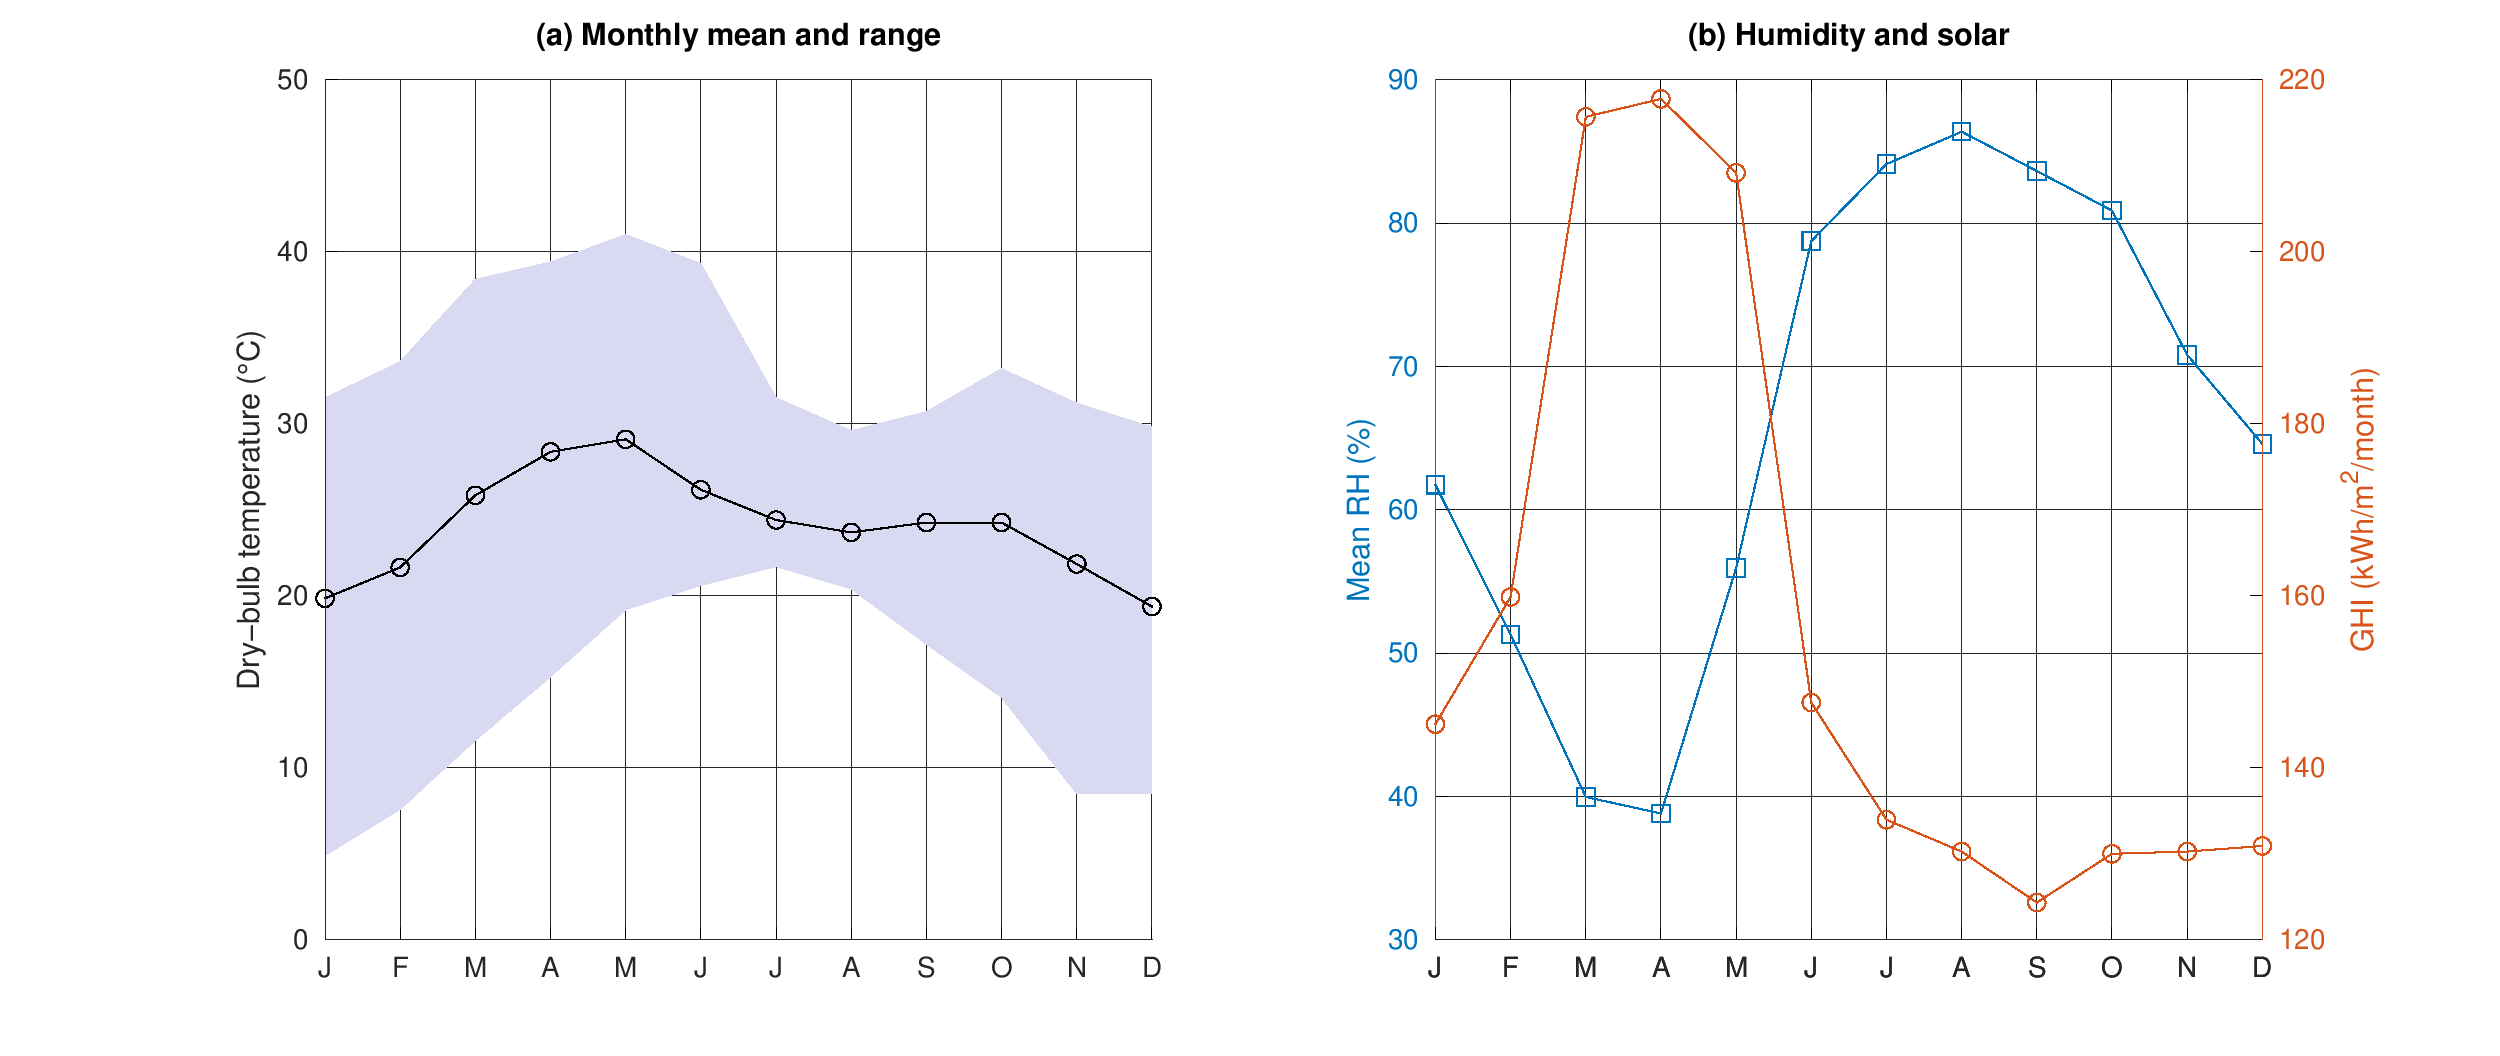
\includegraphics[width=\linewidth]{Fig01_climate.png}
\caption{ISHRAE typical-year climate for Pune: (a) monthly mean and range of dry-bulb
temperature; (b) mean relative humidity and monthly global horizontal irradiation.}
\label{fig:climate}
\end{figure}

\begin{figure}[t]\centering
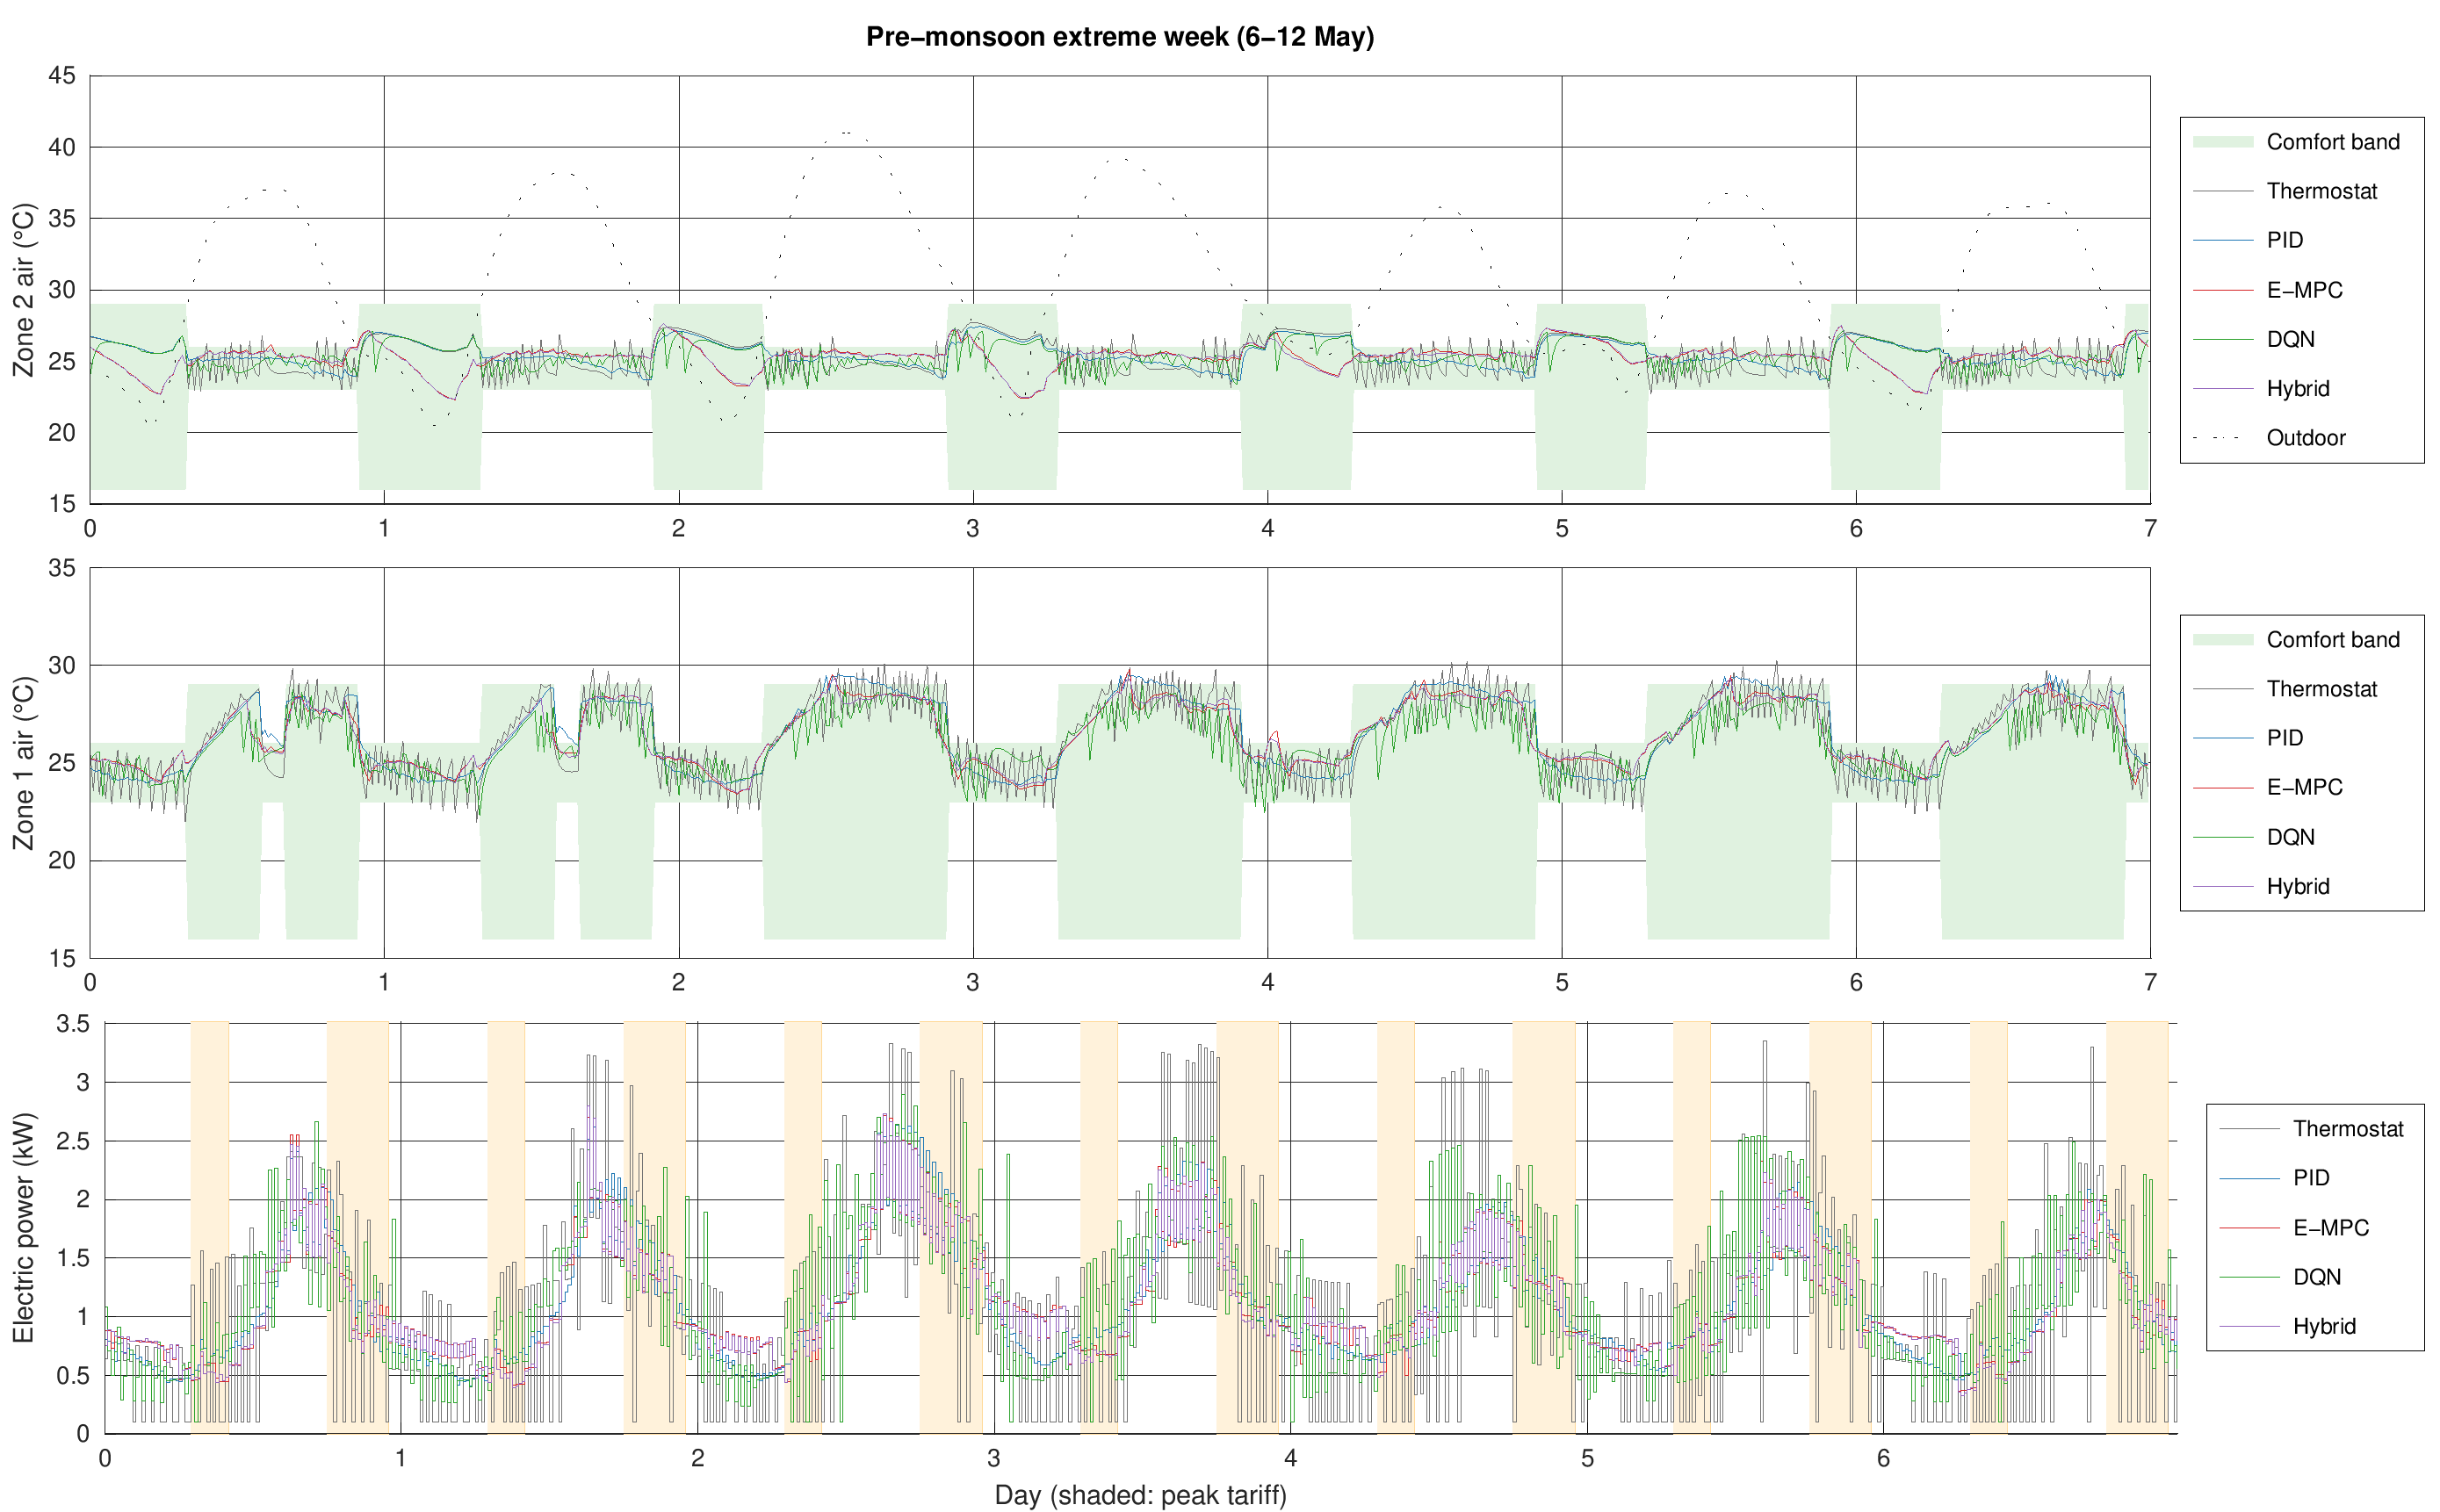
\includegraphics[width=\linewidth]{Fig02a_week_1.png}
\caption{Extreme pre-monsoon week (6--12 May), seed 1. Top: Zone~2 air temperature with
the occupancy-dependent comfort band (shaded) and outdoor temperature. Middle: Zone~1.
Bottom: total electric power, with peak-tariff hours shaded.}
\label{fig:week}
\end{figure}

\subsection{Annual cost, energy and comfort}
Table~\ref{tab:main} and Fig.~\ref{fig:pareto} give the annual results, as the mean
and 95\,\% interval over five seeds.

\textbf{Thermostat: cheapest, but at the cost of comfort.} The thermostat has the
lowest electricity cost (INR~\CostTh) and energy use (\ETh\,kWh). It also has the
largest discomfort (\KhTh\,K\,h) and the lowest share of acceptable occupied zone-hours
(\AccTh\,\%). Most of that discomfort is cooling-induced overcooling (\KhColdTh\,K\,h):
each unit runs at full capacity until the zone is 0.5\,K below the setpoint, and the
air node's 25-min time constant carries it well below 23\,$^\circ$C. The thermostat
also starts the compressor about \StartsRatioTh{} times more often than the Hybrid
controller.

\textbf{The four modulating controllers.} All four cut discomfort by 71--83\,\%
compared with the thermostat, and they spend 3--7\,\% more on electricity to do it.
\begin{itemize}
  \item \textbf{Hybrid} has the lowest discomfort (\KhHyb\,K\,h, \AccHyb\,\% acceptable)
        and is the cheapest of the four (INR~\CostHyb). Against PID it reduces cost by
        \RelHybPidCost\,\% and discomfort by \RelHybPidKh\,\%. Against E-MPC it reduces
        cost by \RelHybMpcCost\,\% and discomfort by \RelHybMpcKh\,\%.
  \item \textbf{E-MPC} costs \RelMpcPidCost\,\% less than PID, with discomfort that is
        \RelMpcPidKh\,\% lower (\KhMpc\ vs \KhPid\,K\,h).
  \item \textbf{DQN} (shielded) lies between PID and E-MPC on cost (INR~\CostDqn) and
        matches E-MPC on discomfort (\KhDqn\,K\,h). It is the only controller whose
        outcome varies materially between seeds (cost $\pm$\CostDqnCI, discomfort
        $\pm$\KhDqnCI), reflecting differences between training runs.
\end{itemize}
The seed intervals of the other controllers are narrow: sensor noise and forecast
errors change annual cost by less than 0.1\,\%.

\begin{table}[t]\centering\small
\caption{Annual results, mean $\pm$ 95\,\% CI over five seeds. Discomfort counts
occupied overheating plus cooling-induced overcooling (K\,h); "acceptable" is the
share of occupied zone-hours without either. $\Delta$cost is relative to the
thermostat.}\label{tab:main}
% generated by aggregate_results.m -- mean +/- 95% CI over 5 seeds
\begin{tabular}{lrrrrrrr}
\hline
Controller & Energy (kWh) & Cost (INR) & $\Delta$cost & Discomfort (K\,h) & Acceptable (\%) & RMSE (K) & Peak (kW)\\
\hline
Thermostat & 5028 $\pm$ 1 & 36950 $\pm$ 8 & -- & 1101.5 $\pm$ 3.2 & 82.7 $\pm$ 0.1 & 1.17 $\pm$ 0.00 & 3.38 $\pm$ 0.01\\
PID & 5403 $\pm$ 0 & 39460 $\pm$ 3 & +6.8\% & 315.3 $\pm$ 0.5 & 94.8 $\pm$ 0.0 & 0.75 $\pm$ 0.00 & 2.69 $\pm$ 0.04\\
E-MPC & 5243 $\pm$ 3 & 38306 $\pm$ 26 & +3.7\% & 250.6 $\pm$ 2.2 & 95.7 $\pm$ 0.0 & 0.99 $\pm$ 0.00 & 2.78 $\pm$ 0.07\\
DQN & 5273 $\pm$ 112 & 38799 $\pm$ 682 & +5.0\% & 259.2 $\pm$ 53.8 & 94.3 $\pm$ 0.8 & 0.90 $\pm$ 0.04 & 3.32 $\pm$ 0.07\\
Hybrid & 5198 $\pm$ 1 & 38005 $\pm$ 14 & +2.9\% & 185.1 $\pm$ 1.1 & 96.1 $\pm$ 0.0 & 0.99 $\pm$ 0.00 & 2.78 $\pm$ 0.10\\
\hline
\end{tabular}

\end{table}

\begin{figure}[t]\centering
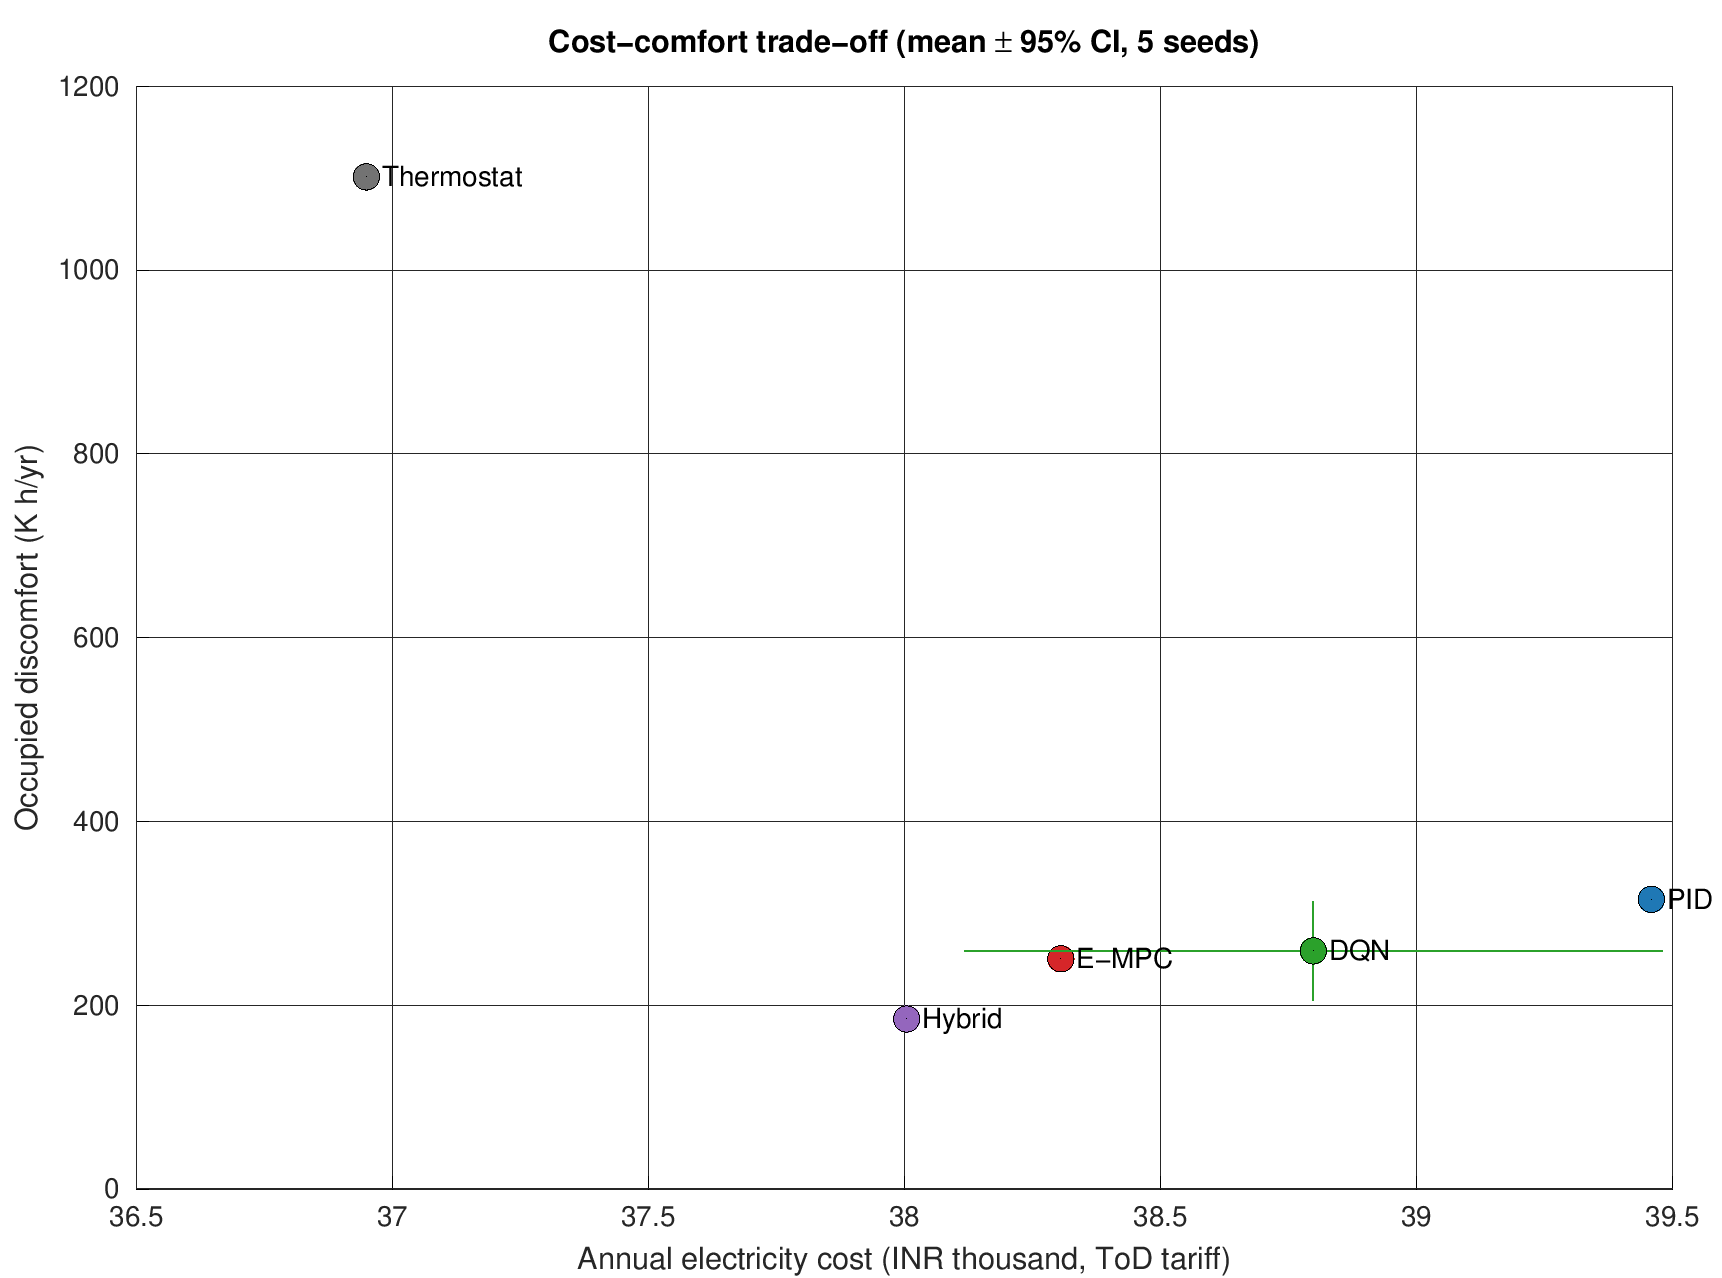
\includegraphics[width=0.62\linewidth]{Fig05_pareto.png}
\caption{Annual ToD electricity cost versus occupied discomfort (mean $\pm$ 95\,\% CI over
five seeds).}\label{fig:pareto}
\end{figure}

\paragraph{Paired daily comparisons.}
These use seed~1 with a block bootstrap and the Wilcoxon signed-rank test.
\begin{itemize}
  \item Hybrid vs PID: cost INR~$\PairHybridPidCost${}
        [$\PairHybridPidCostLo$, $\PairHybridPidCostHi$], $p\PairHybridPidCostP$; discomfort
        $\PairHybridPidKh$\,K\,h [$\PairHybridPidKhLo$, $\PairHybridPidKhHi$],
        $p\PairHybridPidKhP$. Both differences are significant.
  \item Hybrid vs E-MPC: cost INR~$\PairHybridMpcCost${}
        [$\PairHybridMpcCostLo$, $\PairHybridMpcCostHi$]; discomfort $\PairHybridMpcKh$\,K\,h
        [$\PairHybridMpcKhLo$, $\PairHybridMpcKhHi$]; both $p\PairHybridMpcCostP$. Both
        differences are significant.
  \item E-MPC vs PID: the discomfort difference is not significant
        ($p=\PairMpcPidKhP$), but the cost saving is
        (INR~$\PairMpcPidCost${} [$\PairMpcPidCostLo$, $\PairMpcPidCostHi$]).
\end{itemize}

\subsection{Where the energy goes}
Fig.~\ref{fig:energy} breaks electricity down by month and end use.
\begin{itemize}
  \item The VRF accounts for 61--65\,\% of annual electricity.
  \item The DOAS (fans, energy recovery and the demand-controlled dehumidifying coil)
        uses 1.2--1.3\,MWh, about a quarter of the total, mostly during the monsoon. It
        is the largest load outside the controllers' authority.
  \item The recirculation filter fan adds a constant 0.53\,MWh.
  \item The IEC uses 0.1--0.2\,MWh and runs for 580--1100\,h in the dry pre-monsoon.
        Its runtime depends on the controller, because it is enabled only while
        cooling is requested.
\end{itemize}
Monthly electricity peaks in May at 760--805\,kWh and is lowest in December and January.

\begin{figure}[t]\centering
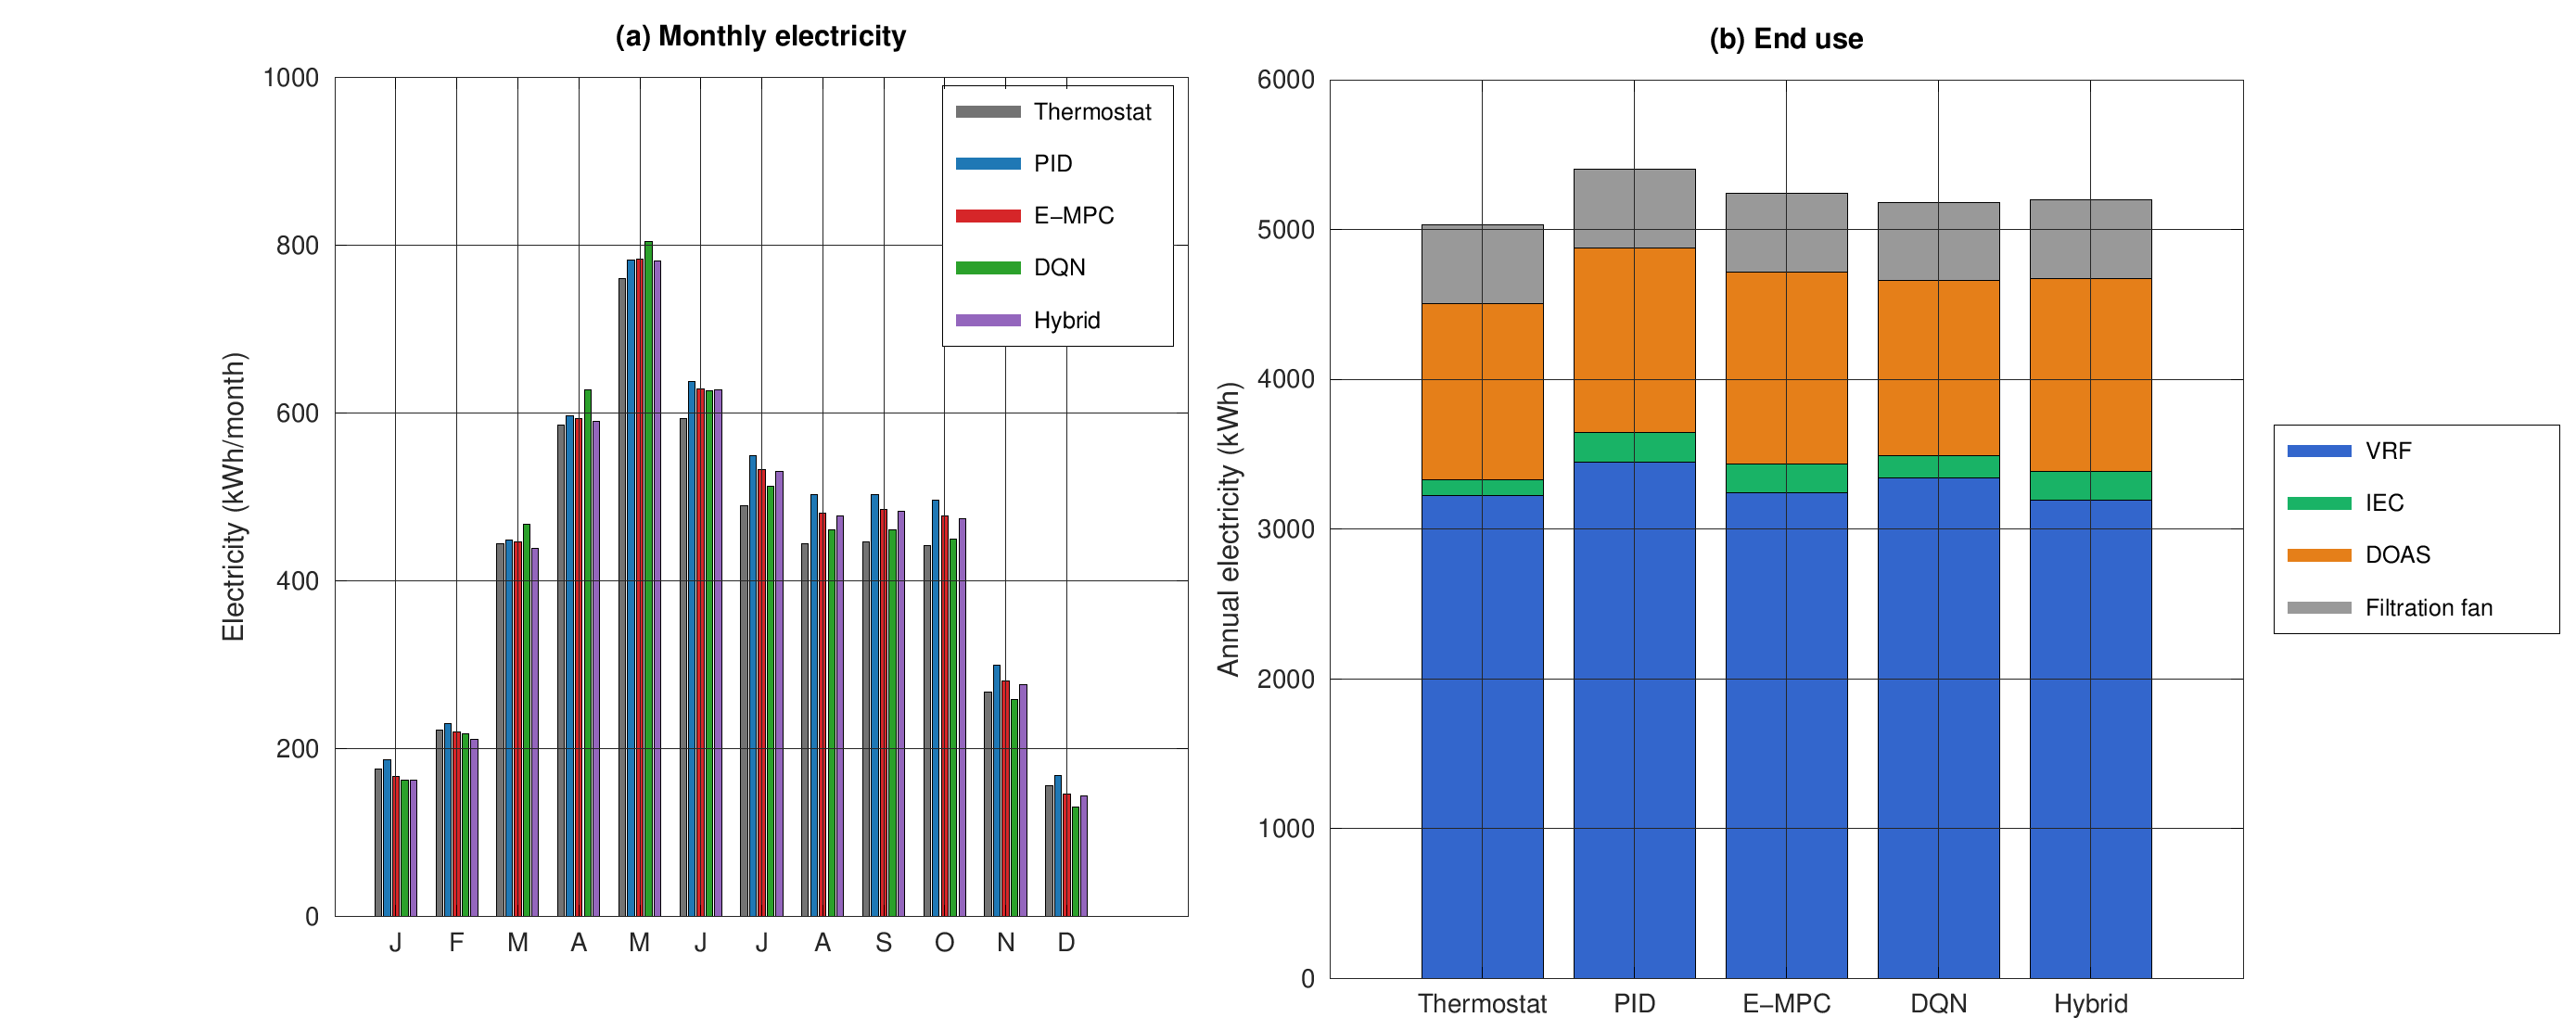
\includegraphics[width=\linewidth]{Fig03_energy.png}
\caption{(a) Monthly electricity (actual monthly sums) and (b) annual end-use split, seed 1.}
\label{fig:energy}
\end{figure}

\subsection{Load shifting under the ToD tariff}
Fig.~\ref{fig:profile} shows the mean daily profile of VRF power for March to June.
E-MPC and Hybrid draw more power than PID between 00:00 and 05:00, when the tariff is
off-peak, and less around 10:00--11:00, so they pre-cool the thermal mass at night.
The share of VRF energy used in peak-tariff hours, however, is almost the same for every
controller (\PeakShareTh--\PeakShareDqn\,\%). The flat-tariff scenario confirms this:
removing the ToD signal changes E-MPC energy use by less than 0.5\,\%
(Section~\ref{sec:sens}). The economic MPC's advantage therefore comes mainly from
temperature-aware efficiency (cooling when the COP is higher) and from riding the upper
comfort bound. It does not come from moving demand out of the 07:00--10:00 and
18:00--23:00 peak windows: all peak-window cooling serves occupied zones, and the
day's stored heat is released from the slab in the evening (Section~\ref{sec:discussion}).

\begin{figure}[t]\centering
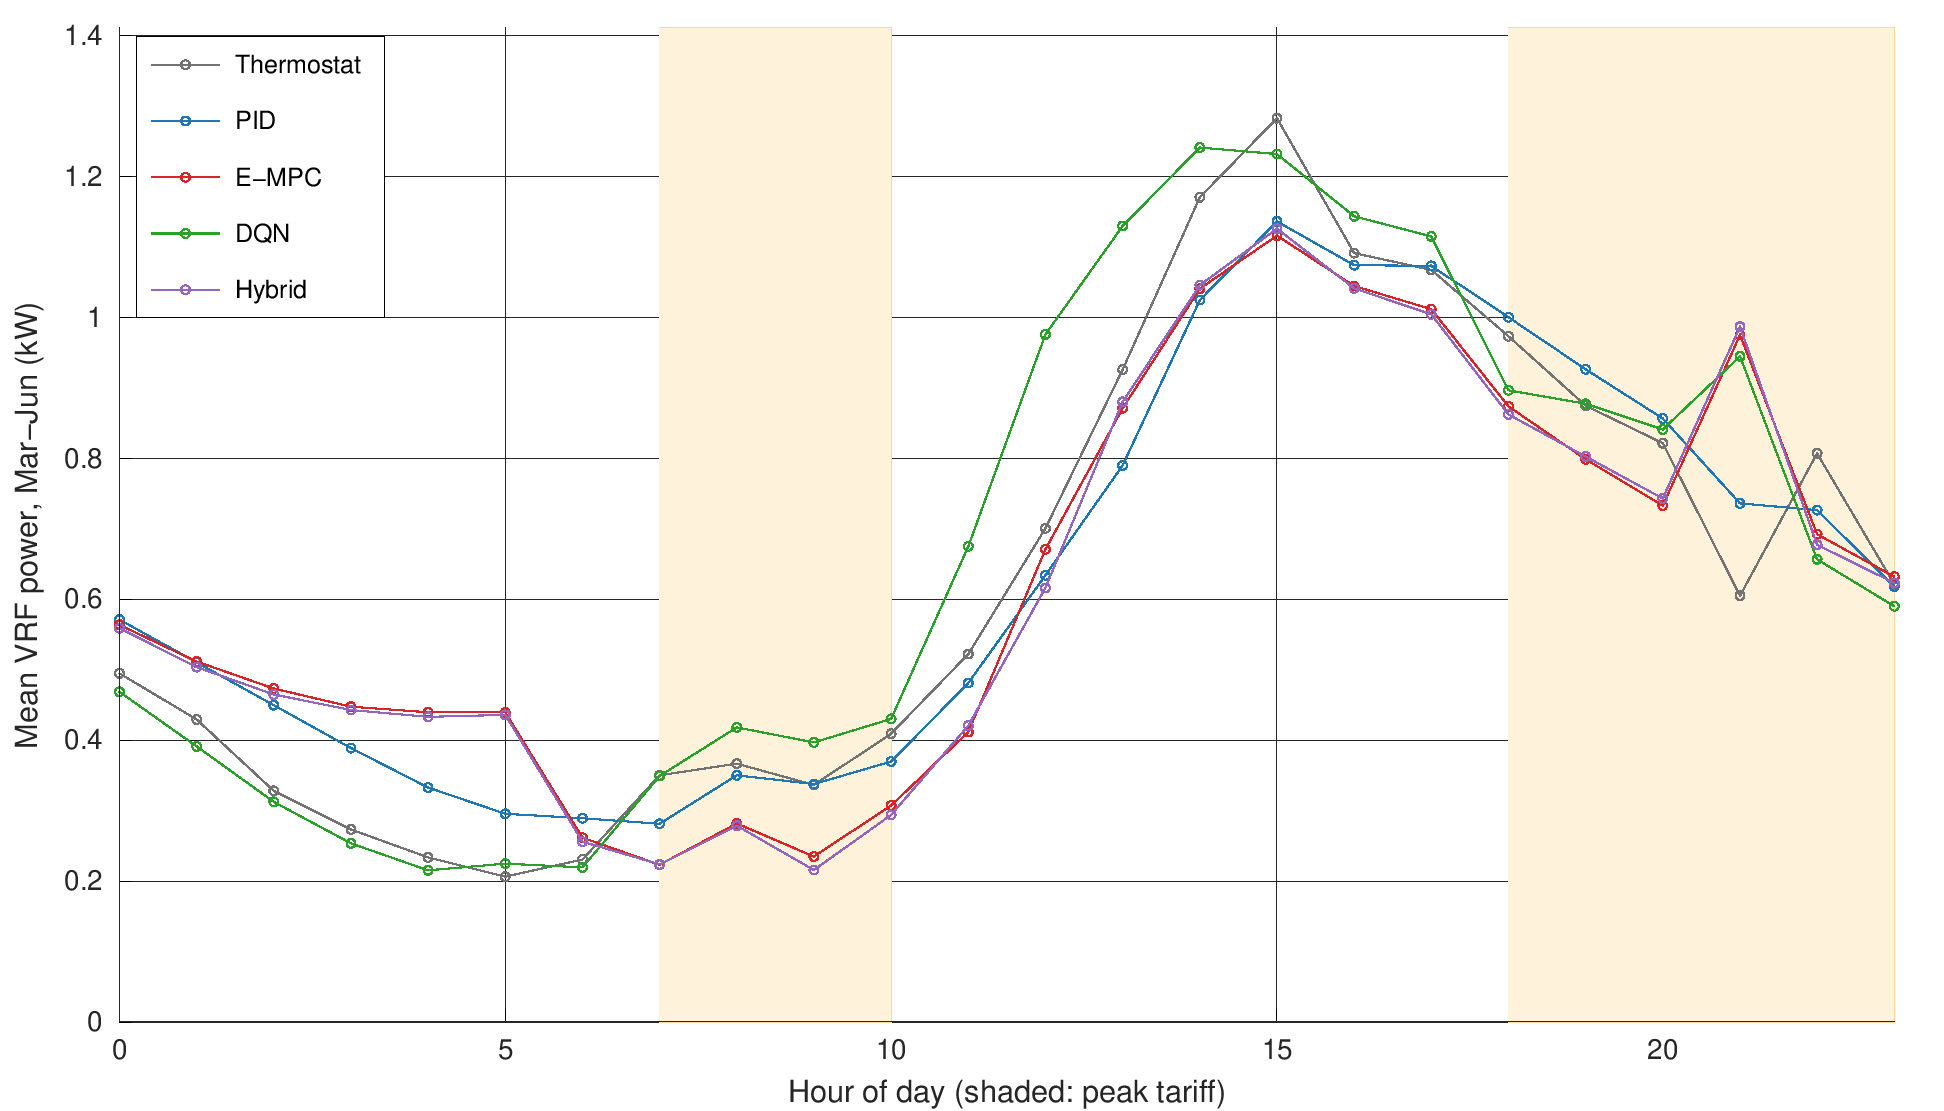
\includegraphics[width=0.7\linewidth]{Fig04_daily_profile.png}
\caption{Mean VRF power by hour of day, March--June, seed 1; peak-tariff hours shaded.}
\label{fig:profile}
\end{figure}

\subsection{Comfort by zone}
Fig.~\ref{fig:comfort}a shows that the ranking holds in every zone. The temperature
distributions in Fig.~\ref{fig:comfort}b show how the controllers differ:
\begin{itemize}
  \item PID concentrates at its 24.5\,$^\circ$C setpoint;
  \item E-MPC and Hybrid concentrate just below 25.5\,$^\circ$C (the band edge minus
        the back-off), which is why they use less energy than PID;
  \item the thermostat and DQN distributions are broad, and the thermostat's has a
        long cold tail.
\end{itemize}

\begin{figure}[t]\centering
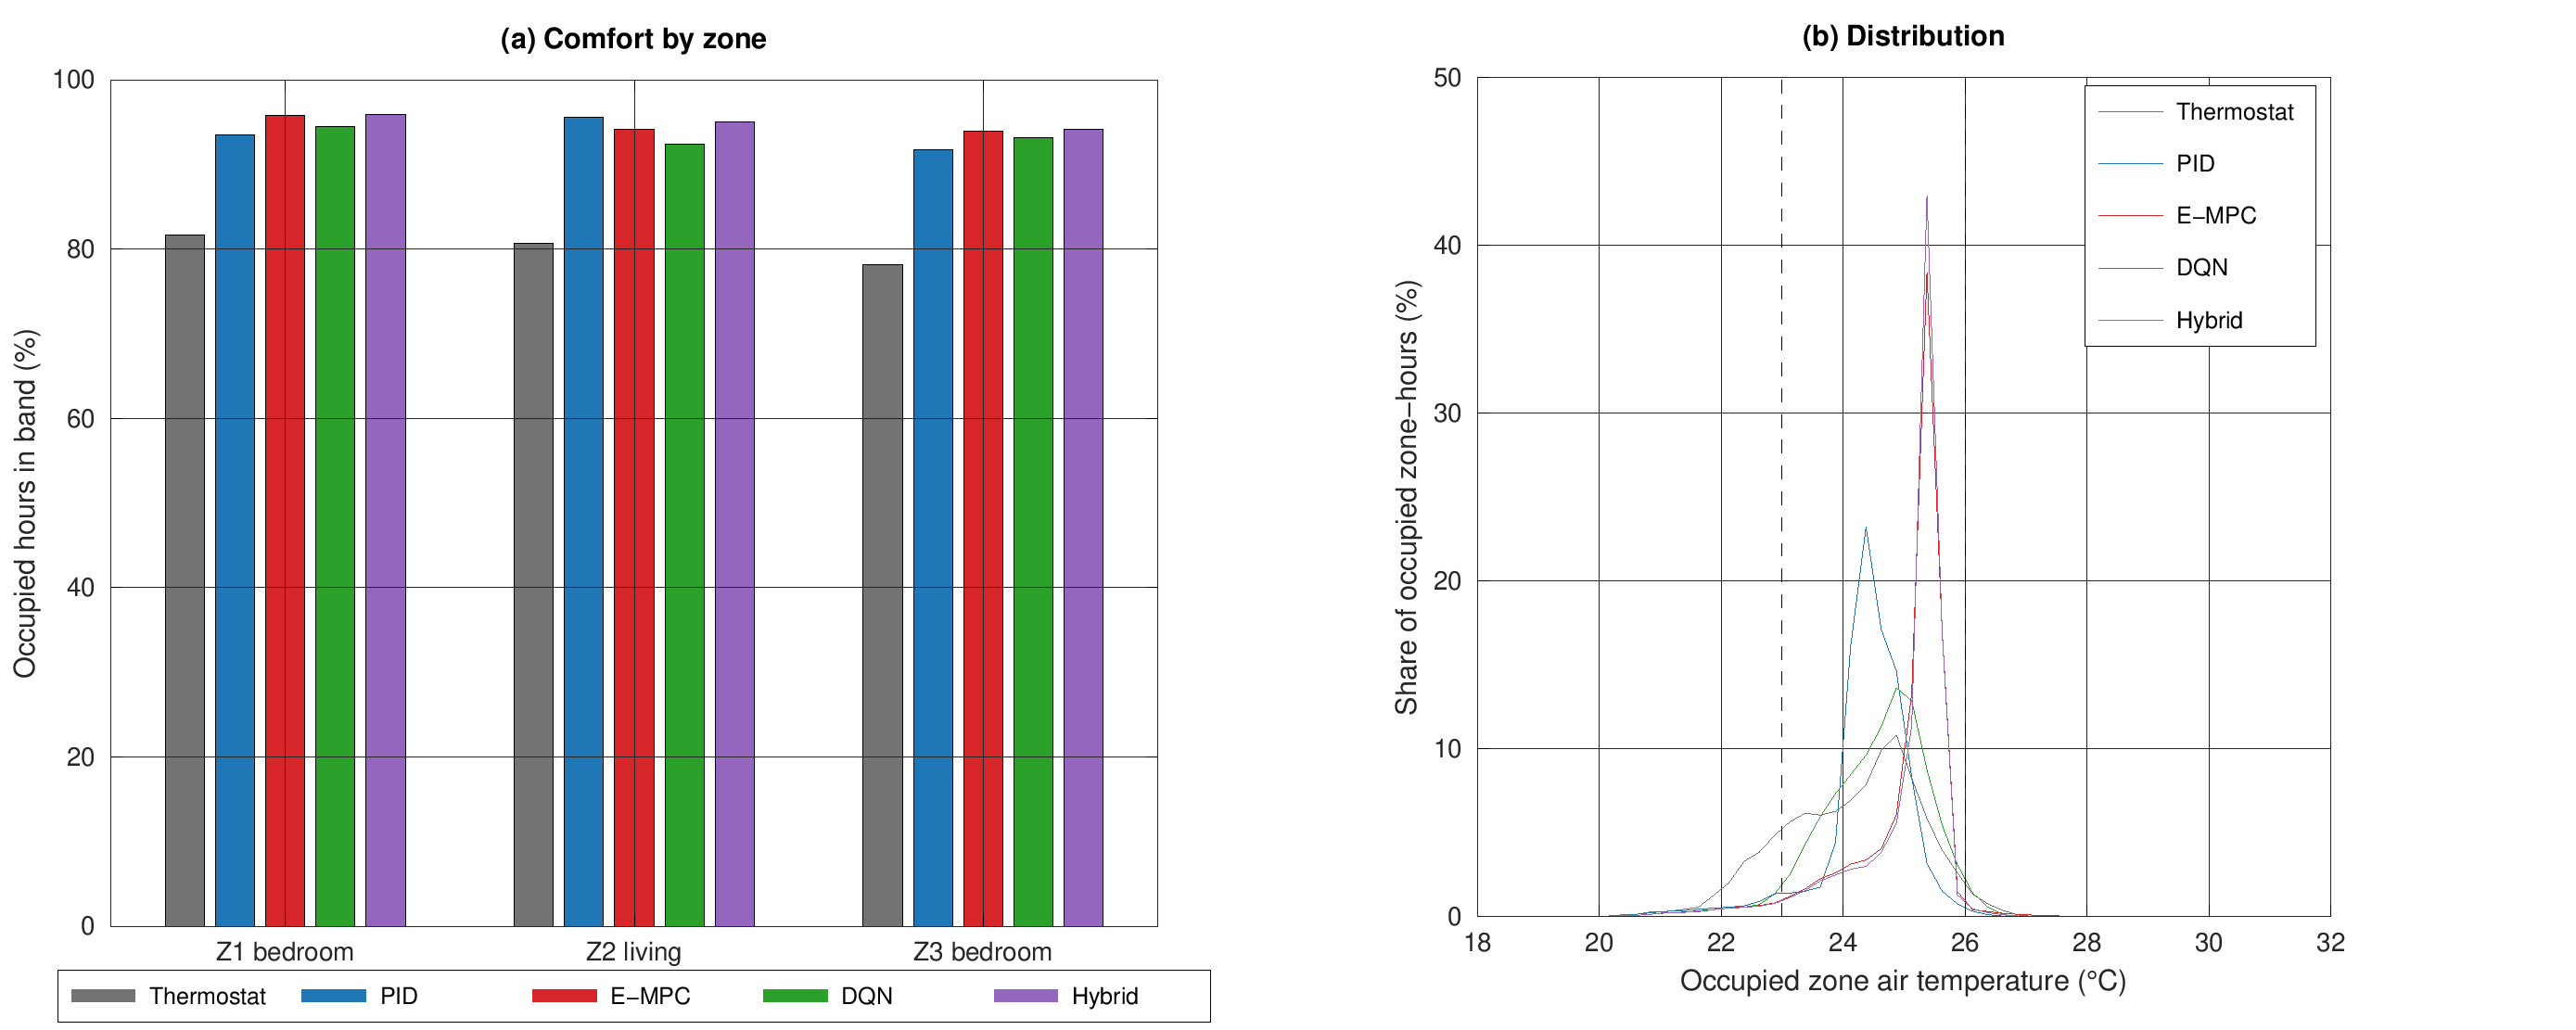
\includegraphics[width=\linewidth]{Fig06_comfort.png}
\caption{(a) Share of occupied hours within the comfort band by zone; (b) distribution of
occupied zone air temperatures (all zones), seed 1.}\label{fig:comfort}
\end{figure}

\subsection{Robustness, sensitivity and ablations}\label{sec:sens}
Table~\ref{tab:sens} and Fig.~\ref{fig:sens} report single-seed results for each
scenario.

\paragraph{Heatwave (+3\,K all year).}
The DQN never saw this weather in training. Cooling cost rises by about a third for all
controllers, and discomfort falls because a warmer winter means less cooling-induced
overcooling. Results:
\begin{itemize}
  \item Hybrid: INR~\SHeatCostHyb, \SHeatKhHyb\,K\,h, still the best on both criteria;
  \item E-MPC: INR~\SHeatCostMpc, \SHeatKhMpc\,K\,h;
  \item PID: INR~\SHeatCostPid, \SHeatKhPid\,K\,h;
  \item DQN: INR~\SHeatCostDqn, \SHeatKhDqn\,K\,h, the most expensive of the
        modulating controllers;
  \item thermostat: \SHeatKhTh\,K\,h.
\end{itemize}
Under sustained heat PID's discomfort falls below E-MPC's. Two tests separate the
possible causes. Giving the E-MPC a perfect model and perfect weather forecasts in the
heatwave year does not help (INR~\SHeatPerfCostMpc, \SHeatPerfKhMpc\,K\,h), so
prediction error is not the cause. Raising the E-MPC back-off from 0.5 to 1.0\,K does
help: discomfort falls to \SHeatBackKhMpc\,K\,h, close to PID's \SHeatKhPid\,K\,h,
at a cost of INR~\SHeatBackCostMpc. The E-MPC loses on comfort because it
deliberately operates close to the upper bound, while PID holds 24.5\,$^\circ$C with
a 1.5\,K margin; under sustained high load, small excursions above a bound that is
barely respected accumulate. With the same 1.0\,K back-off the Hybrid reaches
\SHeatBackKhHyb\,K\,h at INR~\SHeatBackCostHyb. The comfort--cost trade-off is
therefore partly a tuning choice. The shielded DQN transfers to the
hotter year without retraining, but loses its cost advantage over PID.

\paragraph{Thermal mass.}
Halving the effective mass raises discomfort for every controller, because the air
temperature then follows gains more tightly. With half the mass, E-MPC's discomfort
rises to \SMassLoKhMpc\,K\,h and Hybrid's to \SMassLoKhHyb\,K\,h. Doubling the mass
reduces discomfort to \SMassHiKhMpc\ and \SMassHiKhHyb\,K\,h respectively, and lowers
cost. All controllers benefit from more mass; Hybrid remains best on both criteria in
both cases.

\paragraph{Tariff.}
Under a flat tariff, E-MPC uses \SFlatEMpc\,kWh, against \SBaseEMpc\,kWh under ToD. That
near-equality confirms that the ToD term barely changes its decisions in this building:
the savings are efficiency gains, not arbitrage. Two further tariffs test whether this
is a property of the building or of the price signal.
\begin{itemize}
  \item \textbf{Steeper three-tier tariff} (INR 4.00/7.15/14.30 per kWh, a 3.6:1
        peak-to-off-peak ratio): the share of VRF energy in peak hours falls from about
        34\,\% to \SSteepPkShMpc{} (E-MPC) and \SSteepPkShHyb{} (Hybrid), against
        \SSteepPkShPid{} for PID and \SSteepPkShTh{} for the thermostat. A steep enough
        signal does move about 5 percentage points of cooling out of the peak windows.
  \item \textbf{Actual MSEDCL residential structure} (flat INR 7.15 per kWh with a
        INR 0.80 rebate between 09:00 and 17:00): annual costs are INR~\SMsedclCostTh{}
        (thermostat), \SMsedclCostPid{} (PID), \SMsedclCostMpc{} (E-MPC),
        \SMsedclCostDqn{} (DQN) and \SMsedclCostHyb{} (Hybrid), with discomfort
        unchanged from the base case. The Hybrid remains the most comfortable and is
        still 4.4\,\% cheaper than PID, but the DQN is now marginally (0.1\,\%)
        cheaper than the Hybrid. The DQN places 45\,\% of its VRF energy in rebate hours,
        against about 41\,\% for the thermostat, E-MPC and Hybrid; the E-MPC and Hybrid
        do not exploit the small rebate.
\end{itemize}

\paragraph{Information.}
Removing the mismatch changes the plant itself, which then has the nominal, smaller
gains. Costs therefore fall for every controller, including the thermostat
(INR~\SNoMisCostTh). E-MPC falls to INR~\SNoMisCostMpc{} and \SNoMisKhMpc\,K\,h, and
Hybrid to INR~\SNoMisCostHyb{} and \SNoMisKhHyb\,K\,h; the ranking is unchanged. Giving the E-MPC its exact envelope model and perfect weather forecasts
yields INR~\SPerfCostMpc{} and \SPerfKhMpc\,K\,h, no better than the base case. The
remaining gap comes from features the MPC's linear cost does not represent:
\begin{itemize}
  \item VRF part-load and latent behaviour;
  \item IEC and DOAS heat;
  \item the 15-min dynamics inside each hourly block.
\end{itemize}
The Hybrid's feedback layer is designed to correct these. The ablations below show how
much of the Hybrid's advantage the feedback layer actually provides.

\paragraph{Hybrid ablations.}
Removing the PI layer (safety override kept) gives INR~\SNoPICostHyb{} and
\SNoPIKhHyb\,K\,h. Removing the safety override (PI kept) gives INR~\SNoSafeCostHyb{}
and \SNoSafeKhHyb\,K\,h. The full Hybrid gives INR~\SBaseCostHyb{} and
\SBaseKhHyb\,K\,h, and the E-MPC alone INR~\SBaseCostMpc{} and \SBaseKhMpc\,K\,h.
The PI layer therefore provides essentially all of the cost advantage over E-MPC.
Most (about 70\,\%) of the comfort advantage comes from the E-MPC with the safety
override alone. Each layer contributes a little comfort on top of the other.

\paragraph{Uncertainty in assumed inputs.}
Eleven inputs that were assumed rather than measured were varied together in a
\UqN-sample Latin hypercube (single seed):
\begin{itemize}
  \item wall, roof and glazing U-values;
  \item SHGC;
  \item infiltration;
  \item rated COP;
  \item the part-load curve;
  \item occupants;
  \item internal gains;
  \item thermal mass;
  \item the cooking split.
\end{itemize}
Results:
\begin{itemize}
  \item The Hybrid had the lowest discomfort of the modulating controllers in
        \UqBestKhHyb\,\% of samples and the lowest cost in \UqBestCostHyb\,\%
        (the DQN in the rest).
  \item The Hybrid was both cheaper and more comfortable than PID in \UqDomHP\,\% of
        samples, and than E-MPC in \UqDomHM\,\%.
  \item Its cost difference from PID ranged from $\UqHPcostLo$\,\% to
        $\UqHPcostHi$\,\% (5th--95th percentile; median $\UqHPcostMed$\,\%).
  \item Its cost difference from E-MPC was small but consistent: $\UqHMcostLo$\,\% to
        $\UqHMcostHi$\,\%.
  \item The thermostat was cheapest and least comfortable in every sample.
\end{itemize}
The Hybrid's cost advantage over PID shrinks for lighter, more glazed or poorly
insulated roofs (Spearman $\rho$ = 0.60 for roof U-value, 0.49 for SHGC and $-0.38$
for thermal mass). The ranking of the controllers is therefore robust to the assumed
inputs; the size of the saving is not.

\paragraph{MPC horizon.}
Short horizons do slightly better: 6\,h gives INR~\SHorSixCostMpc{} and
\SHorSixKhMpc\,K\,h; 12\,h gives INR~\SHorTwelveCostMpc{} and \SHorTwelveKhMpc\,K\,h;
24\,h gives INR~\SBaseCostMpc{} and \SBaseKhMpc\,K\,h. With forecast errors that grow
with lead time and hourly move blocking, the extra foresight does not pay off.

\paragraph{DQN design.}
\begin{itemize}
  \item Without the safety shield, the agent cools through much of the winter and
        discomfort rises to \SNoShieldKhDqn\,K\,h, at INR~\SNoShieldCostDqn.
  \item With 3 action levels: INR~\SLevThreeCostDqn, \SLevThreeKhDqn\,K\,h.
  \item With 9 action levels: INR~\SLevNineCostDqn, \SLevNineKhDqn\,K\,h.
\end{itemize}

\begin{figure}[t]\centering
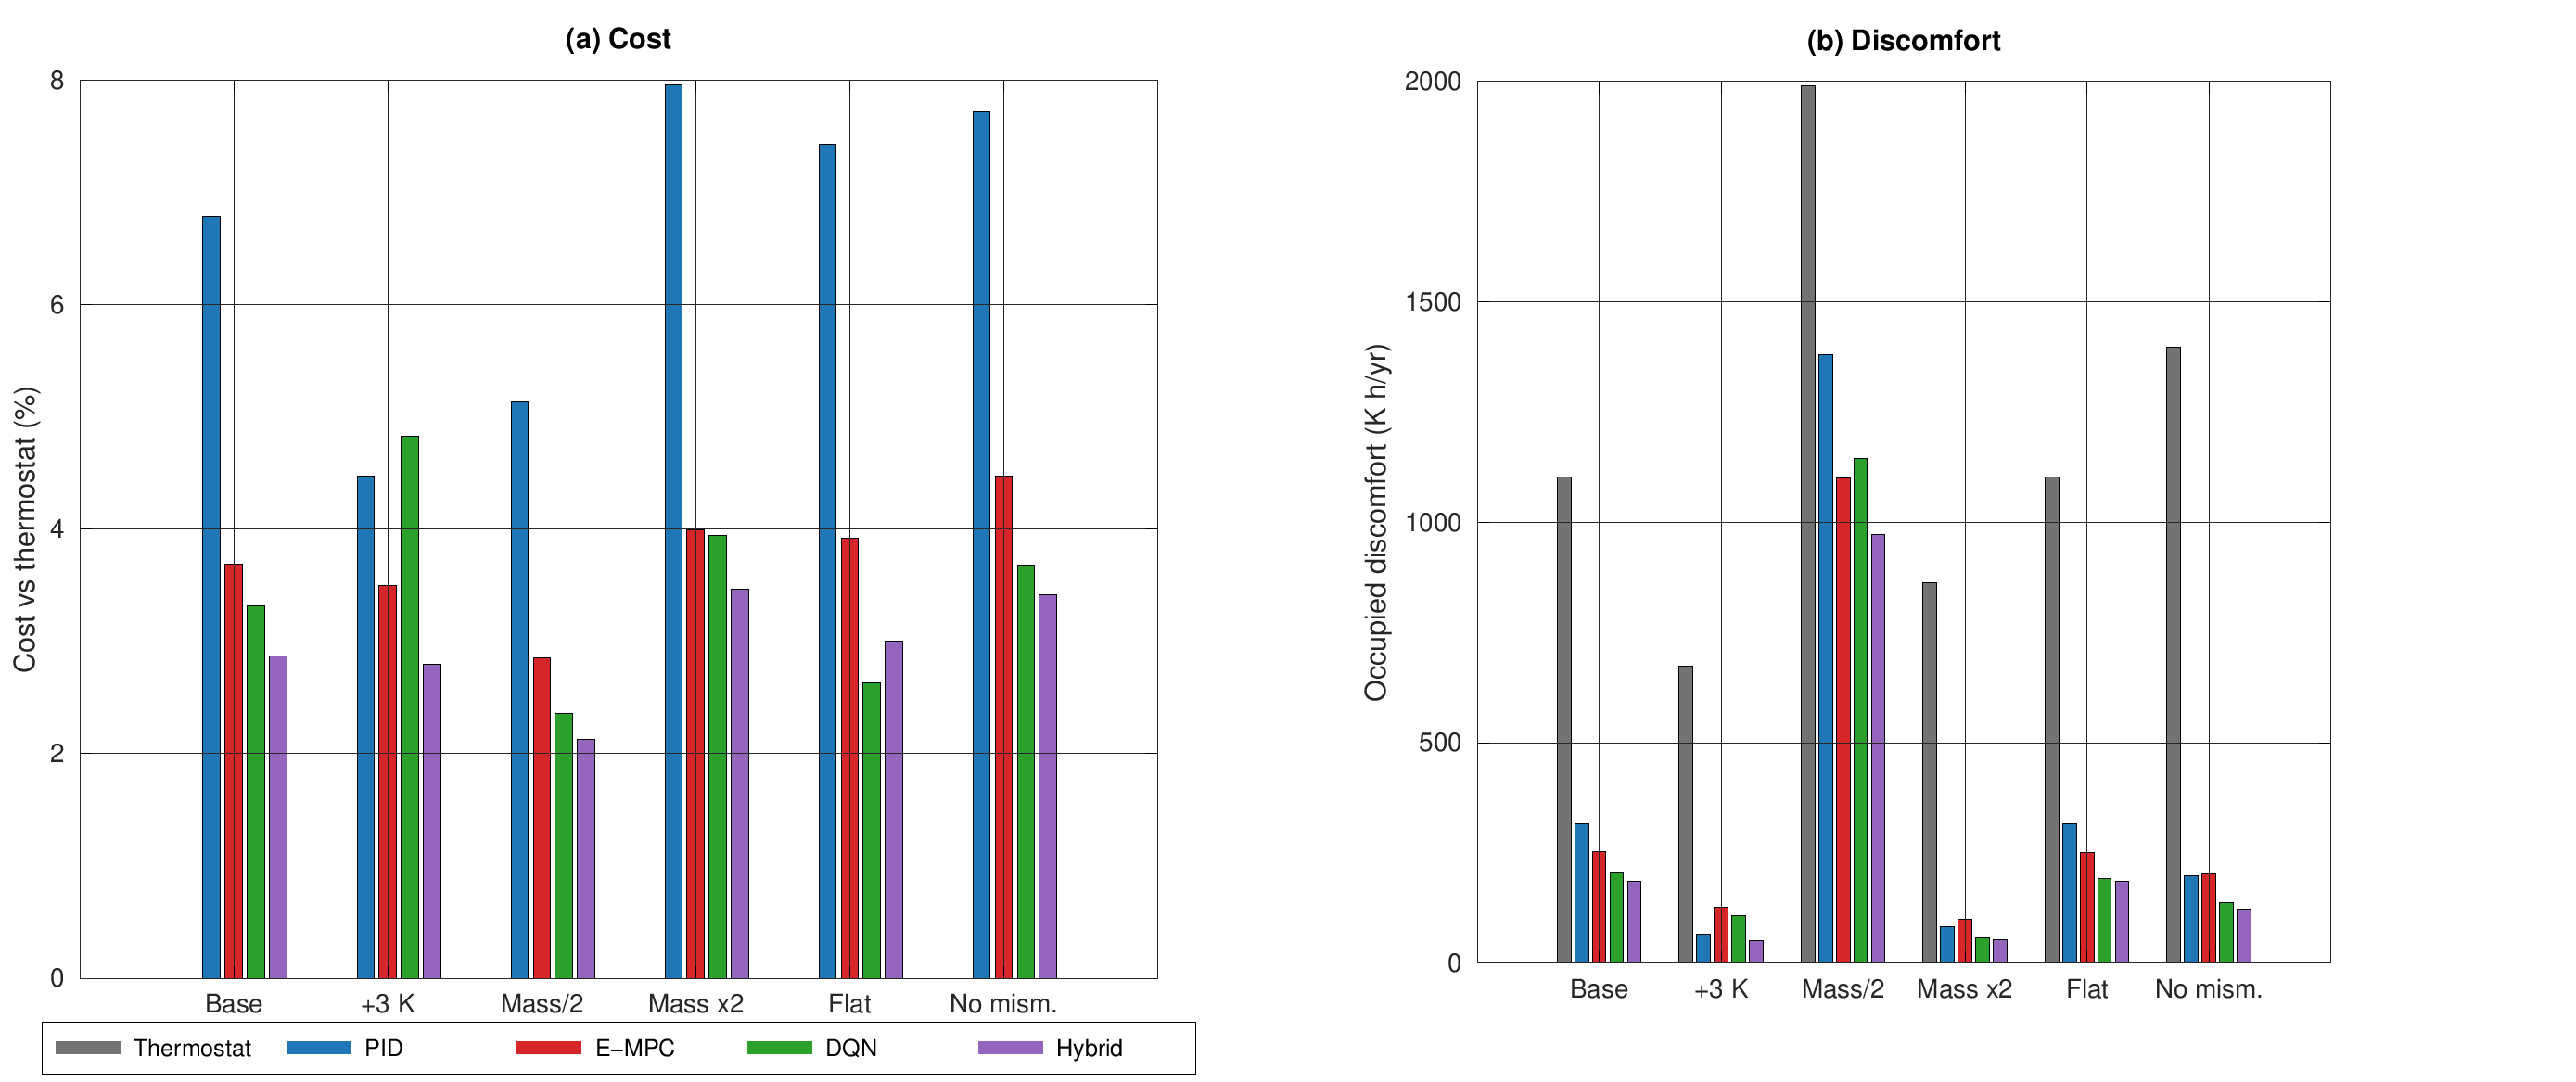
\includegraphics[width=\linewidth]{Fig08_sensitivity.png}
\caption{Sensitivity of (a) annual cost relative to the thermostat and (b) occupied
discomfort across scenarios (seed 1).}\label{fig:sens}
\end{figure}

\subsection{Indoor air quality and ventilation architecture}
CO$_2$ and PM$_{2.5}$ depend on the ventilation and filtration design, not on the
thermal controller (Fig.~\ref{fig:iaq}). Humidity depends on both: controllers that
cool more steadily also remove more moisture.
\begin{itemize}
  \item \textbf{Base design} (continuous 28\,L\,s$^{-1}$ DOAS with MERV-13 filtration
        plus HEPA recirculation), Hybrid controller: mean CO$_2$ \SBaseCoHyb\,ppm; mean
        indoor PM$_{2.5}$ \SBasePmHyb\,$\mu$g\,m$^{-3}$, below the outdoor annual mean
        of about 33\,$\mu$g\,m$^{-3}$; no day above the Indian NAAQS 24-h limit; and
        \SBasePmDHyb\ days above the WHO 24-h guideline, driven by cooking and winter
        outdoor pollution.
  \item \textbf{No recirculation filter}: mean PM$_{2.5}$ rises to
        \SNoFiltPmHyb\,$\mu$g\,m$^{-3}$, above the WHO guideline on every day.
  \item \textbf{CO$_2$}: in the well-mixed whole-dwelling balance it never exceeds
        1000\,ppm in any scenario. Even without mechanical ventilation, 0.5\,ACH of
        infiltration bounds it at about 970\,ppm, against a mean of \SBaseCoHyb\,ppm
        with the DOAS. This is a limitation of the single-volume IAQ model: closed
        bedrooms at night would reach higher concentrations.
  \item \textbf{Humidity}: here the DOAS matters most. Occupied hours with indoor RH
        above 70\,\% are \SVentOffRhHyb\ with no mechanical ventilation, \SVentHumRhHyb\
        with the original humidity-triggered DOAS (60\,L\,s$^{-1}$ in humid weather only),
        and \SBaseRhHyb\ with the demand-controlled dehumidifying DOAS. The original
        design also uses more DOAS energy.
\end{itemize}
The original study reported 160--195\,$\mu$g\,m$^{-3}$ of indoor PM$_{2.5}$ despite HEPA
filtration. That result came from an unstable explicit integration of the mass balance.
With exact integration, recirculating HEPA filtration keeps indoor PM$_{2.5}$ well below
outdoor levels.

\begin{figure}[t]\centering
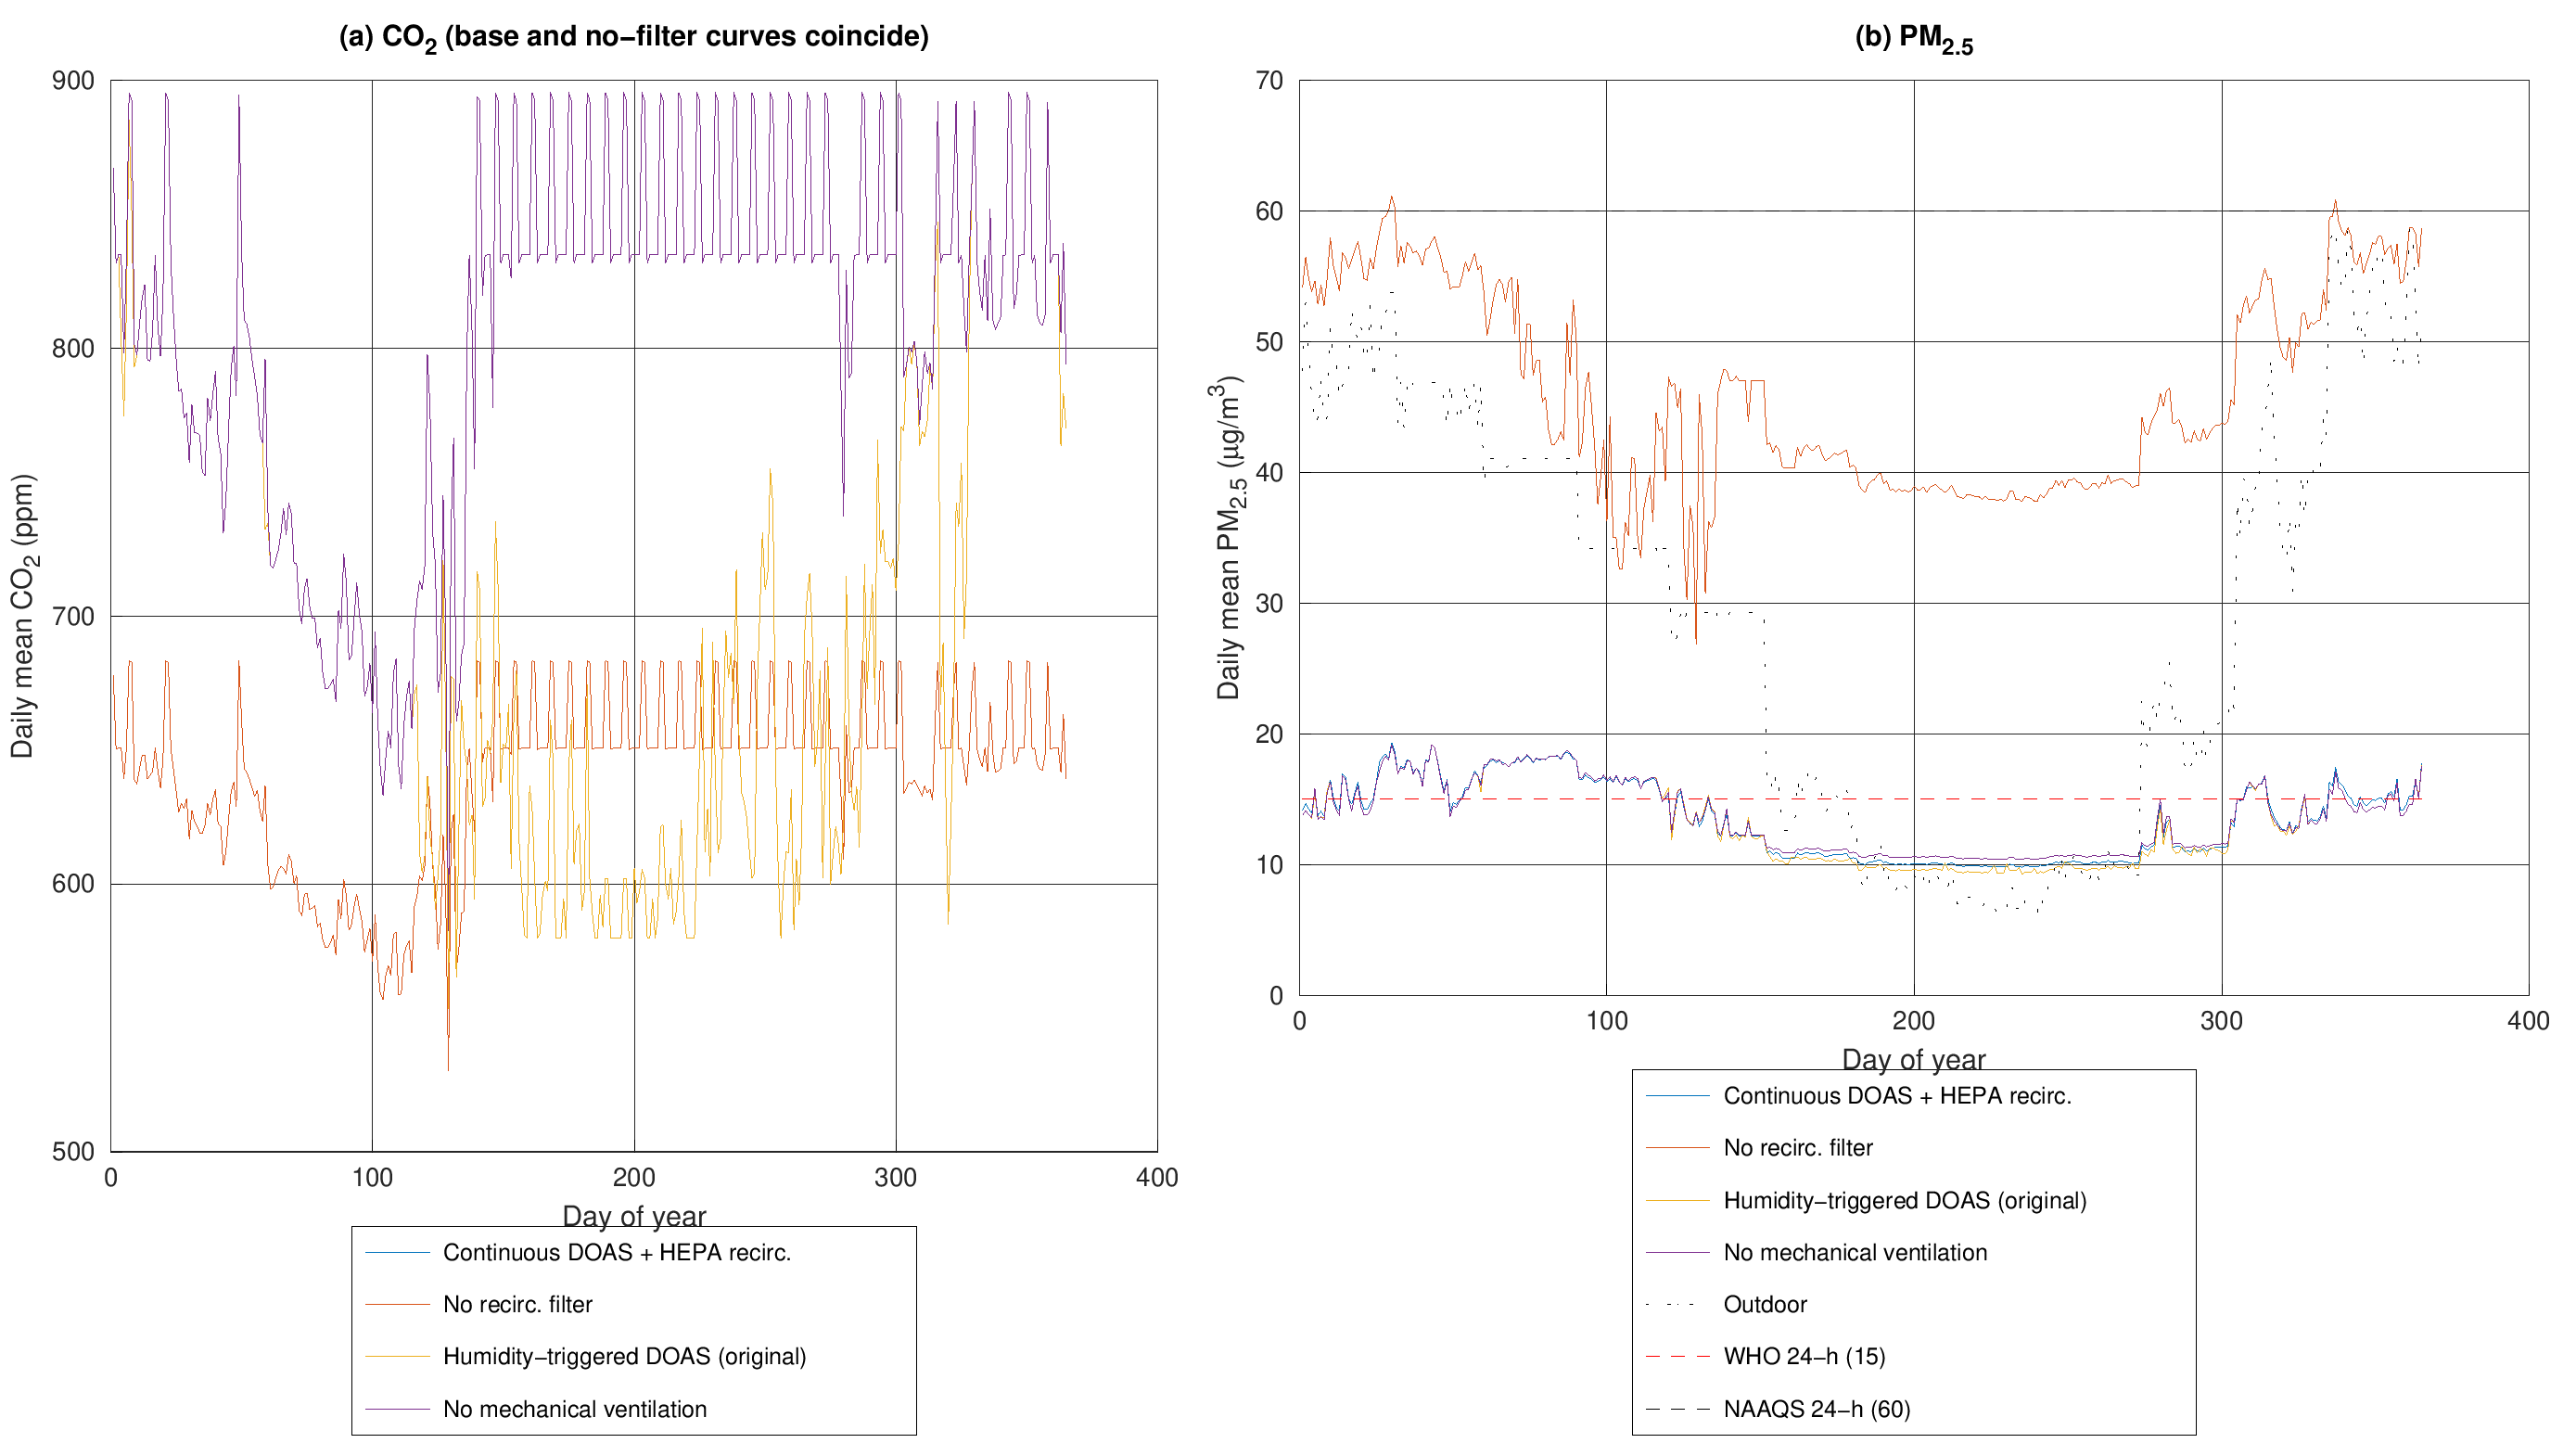
\includegraphics[width=\linewidth]{Fig07_iaq.png}
\caption{Daily mean indoor CO$_2$ (a) and PM$_{2.5}$ (b) for four ventilation/filtration
architectures (Hybrid controller).}\label{fig:iaq}
\end{figure}

\begin{table}[t]\centering\small
\caption{Selected sensitivity and ablation results (seed 1). Cost in INR, discomfort in K\,h.}\label{tab:sens}
\begin{tabular}{lrrrrrrrr}\toprule
 & \multicolumn{2}{c}{PID} & \multicolumn{2}{c}{E-MPC} & \multicolumn{2}{c}{DQN} & \multicolumn{2}{c}{Hybrid}\\
Scenario & Cost & K\,h & Cost & K\,h & Cost & K\,h & Cost & K\,h\\\midrule
Base & \SBaseCostPid & \SBaseKhPid & \SBaseCostMpc & \SBaseKhMpc & \SBaseCostDqn & \SBaseKhDqn & \SBaseCostHyb & \SBaseKhHyb\\
Heatwave +3\,K & \SHeatCostPid & \SHeatKhPid & \SHeatCostMpc & \SHeatKhMpc & \SHeatCostDqn & \SHeatKhDqn & \SHeatCostHyb & \SHeatKhHyb\\
Mass $\times$0.5 & \SMassLoCostPid & \SMassLoKhPid & \SMassLoCostMpc & \SMassLoKhMpc & \SMassLoCostDqn & \SMassLoKhDqn & \SMassLoCostHyb & \SMassLoKhHyb\\
Mass $\times$2 & \SMassHiCostPid & \SMassHiKhPid & \SMassHiCostMpc & \SMassHiKhMpc & \SMassHiCostDqn & \SMassHiKhDqn & \SMassHiCostHyb & \SMassHiKhHyb\\
Flat tariff & \SFlatCostPid & \SFlatKhPid & \SFlatCostMpc & \SFlatKhMpc & \SFlatCostDqn & \SFlatKhDqn & \SFlatCostHyb & \SFlatKhHyb\\
No mismatch & \SNoMisCostPid & \SNoMisKhPid & \SNoMisCostMpc & \SNoMisKhMpc & \SNoMisCostDqn & \SNoMisKhDqn & \SNoMisCostHyb & \SNoMisKhHyb\\
Perfect info & -- & -- & \SPerfCostMpc & \SPerfKhMpc & -- & -- & \SPerfCostHyb & \SPerfKhHyb\\
Horizon 6\,h & -- & -- & \SHorSixCostMpc & \SHorSixKhMpc & -- & -- & \SHorSixCostHyb & \SHorSixKhHyb\\
Horizon 12\,h & -- & -- & \SHorTwelveCostMpc & \SHorTwelveKhMpc & -- & -- & \SHorTwelveCostHyb & \SHorTwelveKhHyb\\
\bottomrule\end{tabular}
\end{table}


\section{Discussion}\label{sec:discussion}

\paragraph{Advanced control buys comfort first, and savings second.}
Against a realistic split-AC thermostat, none of the modulating controllers saves money
in this dwelling. The thermostat's low cost is not efficiency: it comes from short,
full-capacity bursts that overshoot below the comfort band (\KhColdTh\,K\,h of
cooling-induced overcooling) and from about \StartsRatioTh{} times more compressor
starts, and its 15-min peak demand is 21--26\,\% higher than that of PID, E-MPC and
Hybrid. Studies that report large savings against weak or non-modulating baselines
should therefore be read with care. The original version of this study is an example:
its rule-based baseline cooled regardless of indoor temperature. The fair comparison is
between controllers that deliver similar comfort. On that basis the Hybrid controller
is \RelHybPidCost\,\% cheaper than SIMC-tuned PID and has \RelHybPidKh\,\% less
discomfort. Both differences are statistically significant, and both hold under
heatwave, thermal-mass and tariff variations.

\paragraph{Why the Hybrid controller helps.}
The economic MPC finds the cheap operating point: it keeps occupied zones just inside
the upper comfort bound and pre-cools the slab at night when that pays. It does so with
hourly decisions from a linear model that is about 10--15\,\% wrong and from imperfect
forecasts. The ablations show that the Hybrid's two lower layers do different jobs.
\begin{itemize}
  \item The 15-min PI layer supplies essentially all of the cost saving over E-MPC.
  \item Most of the comfort gain comes from the E-MPC with the safety override alone,
        which forces near-full capacity in an occupied zone that exceeds the band.
\end{itemize}
The perfect-information ablation is consistent with this: a better model and perfect
weather do not close the gap, so the gap comes from features outside the MPC's linear
model and from its choice to run close to the bound. The heatwave back-off test points
the same way. Comfort under sustained heat is governed mainly by how much margin the
controller keeps, not by how well it predicts.

\paragraph{Little ToD arbitrage.}
The ToD tariff barely moves the load in this dwelling, even under an economic MPC with a
24-h horizon:
\begin{itemize}
  \item every kWh of peak-window cooling serves an occupied zone, so it cannot be
        dropped without discomfort (occupied zone-hours fall in the peak windows
        slightly less often than hours in general: 27\,\% against 33\,\%);
  \item the heat stored in the roof slab is released in the afternoon and evening:
        mean slab-to-air heat flow is about 2.5\,kW during 18:00--23:00, against
        1.8\,kW at 10:00--16:00;
  \item the peak-to-off-peak price ratio (1.7) is modest. At 3.6:1 the predictive
        controllers move about 5 percentage points of cooling energy out of the peak
        windows.
\end{itemize}
The night pre-cooling we observe mainly reduces late-morning demand, which falls in a
normal-tariff window. Larger demand shifting would need steeper tariffs than the one tested here,
thermal storage or a roof with more accessible mass. The original study reported
evidence of tariff-driven shifting; with real hourly profiles and costs, that evidence
does not survive.

\paragraph{Reinforcement learning needs engineering to be competitive.}
An unconstrained DQN learned to cool through the winter, because "do nothing" is
rarely rewarded once weather-driven cold is excluded from the penalty. That agent was
uncompetitive. Two changes made the DQN competitive with E-MPC on comfort and with
PID-to-MPC on cost:
\begin{itemize}
  \item a safety shield, with the agent's own proposals stored for learning;
  \item checkpoint selection on a separate validation set.
\end{itemize}
The DQN also needs no model at run time. Its seed-to-seed spread is an order of
magnitude larger than that of the model-based controllers, so a single training run is
not a reliable estimate of performance. This supports the protocol used here: several
seeds, a validation set separate from the test year, and robustness checks on weather
not seen in training.

\paragraph{IAQ is decided by design, not by the thermostat logic.}
Indoor CO$_2$ and PM$_{2.5}$ are essentially identical across thermal controllers. They
are governed by the ventilation rate and the filtration architecture: the recirculating
HEPA filter alone reduces mean PM$_{2.5}$ more than threefold. Humid hours are where
design and control interact. The demand-controlled dehumidifying DOAS cuts occupied
hours above 70\,\% RH by about a factor of seven compared with no mechanical
ventilation, and the steadier modulating controllers remove more moisture than the
thermostat. The DOAS (fans and coil) uses about a quarter of annual electricity in this
climate. That load deserves its own optimisation, for example demand-controlled
ventilation or a combined IAQ-thermal MPC.

\paragraph{Practical implications.}
For Indian homes with inverter VRF or multi-split systems:
\begin{enumerate}
  \item Modulating control in place of thermostat on/off is the largest gain. It
        delivers comfort and fewer compressor starts, and with PID or the model-based
        controllers about 18\,\% lower peak demand.
  \item A hybrid MPC plus feedback architecture adds a further 3--4\,\% cost reduction
        over well-tuned PID at better comfort.
  \item Ventilation and filtration design decide IAQ and should be treated as a design
        variable of equal standing.
\end{enumerate}
The computational cost of the MPC (\MsMpc\,ms per hourly solve in interpreted
MATLAB/Octave) is compatible with an embedded gateway.

\section{Limitations}\label{sec:limits}
\begin{itemize}
\item \textbf{Simulation only, one dwelling, one typical year.} The plant is a reduced-order
RC model. It has not been calibrated against measurements or cross-validated against a
detailed whole-building simulation. An EnergyPlus model with the same geometry,
constructions, gains and EPW file is released with the code
(\texttt{validation/energyplus}), together with a script that compares free-floating
temperatures and ideal cooling loads, but that comparison had not been run when this
paper was written. The
absolute energy figures should therefore be read as indicative; the comparisons
between controllers, made on identical inputs, are more robust. Cross-validation
against EnergyPlus is the most important next step.
\item \textbf{Assumed inputs.} Envelope properties, gains, occupancy and equipment
performance are assumed. A 40-sample variation of eleven of them leaves the controller
ranking unchanged but changes the size of the savings (Section~\ref{sec:sens}).
\item \textbf{Tuning on the evaluation year.} The E-MPC weights and back-off, the
Hybrid gains and the DQN hyper-parameters were chosen during development by running on
the same typical year that is used for evaluation. The DQN's validation weeks are also
drawn from that year. The reported margins may therefore be slightly optimistic for an
unseen year; the heatwave case is a partial out-of-sample test.
\item \textbf{Assumed equipment curves.} The VRF rated COP, the part-load curve and the
IEC effectiveness are generic values, not manufacturer data. The released configuration
file allows them to be replaced.
\item \textbf{Representative outdoor PM$_{2.5}$.} The outdoor series is a monthly--diurnal
profile, not measured data. The IAQ results are therefore comparisons between
architectures, not exposure estimates. Hourly CPCB monitoring data for Pune should
replace it.
\item \textbf{Single-volume IAQ.} CO$_2$, PM$_{2.5}$ and moisture are modelled as one
well-mixed volume. Bedrooms with closed doors at night would see higher CO$_2$ than the
whole-dwelling value reported here.
\item \textbf{Dry-bulb comfort.} The comfort band is a static 23--26\,$^\circ$C. Indoor
humidity is reported separately rather than combined into PMV or an adaptive (IMAC)
index.
\item \textbf{Deterministic schedules.} Occupancy, internal gains and cooking follow fixed
weekday and weekend profiles, and occupants cannot override the controller.
\item \textbf{DQN scope.} One value-based algorithm with a discrete action set, trained
in simulation on perturbed copies of the same typical year. Policy-gradient and
continuous-action methods, and training on multiple measured years, were not tested.
\item \textbf{No heating.} The dwelling has no heating, so winter cold is outside the
controllers' authority. It is excluded from the discomfort metric through the
free-floating reference.
\item \textbf{Economics.} The main three-tier ToD tariff is hypothetical, not a published
MSEDCL schedule. The actual MSEDCL residential structure, a flat tariff and a steeper
tariff are tested as sensitivities. One national grid emission factor is used
(CEA, 0.727\,kgCO$_2$/kWh for FY2023--24). Demand charges and tariff revisions are not modelled.
\end{itemize}

\section{Conclusions}\label{sec:conclusion}
This year-long, multi-seed benchmark of residential cooling control for a Pune
apartment supports five conclusions.
\begin{enumerate}
\item With a realistic thermostat as the baseline and a fair discomfort metric,
      advanced controllers pay off mainly in comfort and fewer compressor starts, and
      (except the DQN) in lower peak demand. They do not reduce cost relative to the
      thermostat.
\item Among controllers that deliver good comfort, the hierarchical Hybrid (economic MPC
      with a PI correction layer and safety override) is best. It costs
      \RelHybPidCost\,\% less than SIMC-tuned PID and \RelHybMpcCost\,\% less than
      E-MPC, with \RelHybPidKh\,\% and \RelHybMpcKh\,\% less discomfort respectively.
      The ranking holds under a +3\,K heatwave, thermal mass, the tested tariffs (on comfort) and
      a \UqN-sample variation of eleven assumed inputs. The size of the saving over
      PID varies with the inputs ($\UqHPcostLo$\ to $\UqHPcostHi$\,\%). The PI layer
      provides the cost saving, and the safety override provides most of the
      comfort gain.
\item A DQN with a safety shield, multi-seed training and a separate validation set is
      competitive. Without the shield it is not, and its performance varies with the
      training seed.
\item A hypothetical three-tier ToD tariff with a 1.7:1 price ratio produces little load
      shifting, because peak-window cooling serves occupied zones and coincides with
      heat release from the roof slab. A 3.6:1 ratio shifts about 5 percentage points of
      cooling energy. Under the actual MSEDCL residential structure the Hybrid
      remains the most comfortable and 4\,\% cheaper than PID, with the DQN within
      0.1\,\% of it on cost.
\item Indoor air quality depends on ventilation and filtration design, not on the
      thermal controller. Recirculating HEPA filtration keeps PM$_{2.5}$ well below
      outdoor levels. A demand-controlled dehumidifying DOAS removes most humid hours,
      at an energy cost of about a quarter of annual electricity that deserves dedicated
      control.
\end{enumerate}
Future work should calibrate the model against measured data or EnergyPlus, add
measured hourly PM$_{2.5}$, use adaptive and humidity-aware comfort metrics, and
co-optimise ventilation with cooling in one MPC.


\section*{Data and code availability}
All code, the weather file and the scripts that generate every table and figure are
openly available at \textcolor{red}{[repository URL / Zenodo DOI]}. The study is
reproduced with \texttt{run\_all.m} in MATLAB (no toolboxes) or GNU Octave.

\section*{Declaration of competing interest}
The authors declare no competing interests.

% Verify every entry (authors, volume, pages, DOI) before submission.
\begin{thebibliography}{99}\small
\bibitem{iea2023} International Energy Agency, Energy Efficiency 2023, IEA, Paris, 2023 (section: Can efficient cooling help manage fast rising electricity demand in India and achieve thermal comfort for all?).
\bibitem{drgona2020} J.~Drgo\v{n}a, J.~Arroyo, I.~Cupeiro Figueroa, D.~Blum, K.~Arendt, D.~Kim, E.~Perarnau Oll\'e, J.~Oravec, M.~Wetter, D.L.~Vrabie, L.~Helsen, All you need to know about model predictive control for buildings, Annual Reviews in Control 50 (2020) 190--232.
\bibitem{yao2021} Y.~Yao, D.K.~Shekhar, State of the art review on model predictive control (MPC) in heating ventilation and air-conditioning (HVAC) field, Building and Environment 200 (2021) 107952.
\bibitem{yu2021} L.~Yu, S.~Qin, M.~Zhang, C.~Shen, T.~Jiang, X.~Guan, A review of deep reinforcement learning for smart building energy management, IEEE Internet of Things Journal 8 (2021) 12046--12063.
\bibitem{sierla2022} S.~Sierla, H.~Ihasalo, V.~Vyatkin, A review of reinforcement learning applications to control of heating, ventilation and air conditioning systems, Energies 15 (2022) 3526.
\bibitem{arroyo2022} J.~Arroyo, C.~Manna, F.~Spiessens, L.~Helsen, Reinforced model predictive control (RL-MPC) for building energy management, Applied Energy 309 (2022) 118346.
\bibitem{mnih2015} V.~Mnih et al., Human-level control through deep reinforcement learning, Nature 518 (2015) 529--533.
\bibitem{vanhasselt2016} H.~van Hasselt, A.~Guez, D.~Silver, Deep reinforcement learning with double Q-learning, Proc. AAAI Conference on Artificial Intelligence 30 (2016).
\bibitem{alshiekh2018} M.~Alshiekh, R.~Bloem, R.~Ehlers, B.~K\"onighofer, S.~Niekum, U.~Topcu, Safe reinforcement learning via shielding, Proc. AAAI Conference on Artificial Intelligence 32 (2018) 2669--2678. doi:10.1609/aaai.v32i1.11797.
\bibitem{skogestad2003} S.~Skogestad, Simple analytic rules for model reduction and PID controller tuning, Journal of Process Control 13 (2003) 291--309.
\bibitem{beck2009} A.~Beck, M.~Teboulle, A fast iterative shrinkage-thresholding algorithm for linear inverse problems, SIAM Journal on Imaging Sciences 2 (2009) 183--202.
\bibitem{wang2024} X.~Wang, B.~Dong, Long-term experimental evaluation and comparison of advanced controls for HVAC systems, Applied Energy 371 (2024) 123706.
\bibitem{biemann2021} M.~Biemann, F.~Scheller, X.~Liu, L.~Huang, Experimental evaluation of model-free reinforcement learning algorithms for continuous HVAC control, Applied Energy 298 (2021) 117164.
\bibitem{manu2016} S.~Manu, Y.~Shukla, R.~Rawal, L.E.~Thomas, R.~de~Dear, Field studies of thermal comfort across multiple climate zones for the subcontinent: India Model for Adaptive Comfort (IMAC), Building and Environment 98 (2016) 55--70.
\bibitem{nbc2005} Bureau of Indian Standards, National Building Code of India 2005, Part 8 Building Services, Section 3: Air conditioning, heating and mechanical ventilation, Cl.~4.4.3 (Inside design conditions), Table~2 (summer design range for air-conditioned occupancies 23--26\,$^\circ$C DB).
\bibitem{ens2018} Bureau of Energy Efficiency, Eco-Niwas Samhita 2018 (Energy Conservation Building Code for Residential Buildings), Part I: Building Envelope.
\bibitem{ashrae622} ASHRAE, ANSI/ASHRAE Standard 62.2, Ventilation and Acceptable Indoor Air Quality in Residential Buildings (whole-dwelling rate $Q_{tot}=0.03A_{floor}+7.5(N_{br}+1)$\,cfm, unchanged since the 2013 edition).
\bibitem{belias2022} E.~Belias, D.~Licina, Outdoor PM2.5 air filtration: optimising indoor air quality and energy, Buildings \& Cities 3 (2022) 186--203. doi:10.5334/bc.153.
\bibitem{who2021} World Health Organization, WHO global air quality guidelines: particulate matter (PM2.5 and PM10), ozone, nitrogen dioxide, sulfur dioxide and carbon monoxide, Geneva, 2021.
\bibitem{cpcb2009} Central Pollution Control Board, National Ambient Air Quality Standards, Notification, 18 November 2009.
\bibitem{merc} Maharashtra Electricity Regulatory Commission, Multi-Year Tariff Order for MSEDCL, Case No.~217 of 2024 (28 March 2025), as modified by the review order of 25 June 2025 (residential ToD rebate of INR 0.80/kWh during solar hours 09:00--17:00 in FY~2025--26, rising to INR 1.00/kWh by FY~2029--30; night rebate removed).
\bibitem{cea} Central Electricity Authority, CO$_2$ Baseline Database for the Indian Power Sector, Version 20.0, User Guide, December 2024 (weighted average emission factor of the Indian grid, FY2023-24: 0.727 tCO$_2$/MWh).
\bibitem{ishrae} ISHRAE, Indian Weather Data for Energy Simulation (ISHRAE/EnergyPlus weather files), Pune 430630.
\end{thebibliography}

\end{document}
